\documentclass[supercite]{Experimental_Report}

\title{~~~~~~数据结构实验~~~~~~}
\author{Eren·Yeager}
%\coauthor{张三、李四}
\school{计算机科学与技术学院}
\classnum{CS}
\stunum{塔塔开!}
%\costunum{U202115631、U202115631}
\instructor{Eren·Yeager} % 该系列实验报告模板有华科大计院教师陈加忠制作
\date{2022年5月15日}

\usepackage{algorithm, multirow}
\usepackage{algpseudocode}
\usepackage{amsmath}
\usepackage{amsthm}
\usepackage{framed}
\usepackage{mathtools}
\usepackage{subcaption}
\usepackage{xltxtra} %提供了针对XeTeX的改进并且加入了XeTeX的LOGO, 自动调用xunicode宏包(提供Unicode字符宏)
\usepackage{bm}
\usepackage{tikz}
\usepackage{tikzscale}
\usepackage{pgfplots}
\usepackage{listings}
\usepackage{xcolor}
\usepackage{fontspec}
\usepackage{subfiles}
%\usepackage{subfigure}
%\usepackage{enumerate}

%%%%%%settings%%%%%%%%%
\pgfplotsset{compat=1.16}
%\setmonofont{Consolas}

\definecolor{mygreen}{rgb}{0,0.6,0}
\definecolor{mygray}{rgb}{0.5,0.5,0.5}
\definecolor{mymauve}{rgb}{0.58,0,0.82}
\lstset{ %
	backgroundcolor=\color{white},   % choose the background color
	basicstyle=\footnotesize\ttfamily,        % size of fonts used for the code
	columns=fullflexible,
	breaklines=true,                 % automatic line breaking only atwhitespace
	captionpos=b,                    % sets the caption-position to bottom
	tabsize=4,
	commentstyle=\color{mygreen},    % comment style
	escapeinside={\%*}{*)},          % if you want to add LaTeX within your code
	keywordstyle=\color{blue},       % keyword style
	stringstyle=\color{mymauve}\ttfamily,     % string literal style
	frame=single,
	rulesepcolor=\color{red!20!green!20!blue!20},
	% identifierstyle=\color{red},
	language=c++,
}


%%%%%伪代码:请参考算法\ref{alg:1},也可以参考算法\ref{alg:2}。%%%%%
%
%\begin{shaded*}\begin{alg}{一个复杂算法}
%		\label{alg:1}
%		\begin{algorithmic}
%			\Input Two numbers $a$ and $b$
%			\Output The sum of $a$ and $b$
%			\Procedure{A-Plus-B}{$a, b$}
%			\If $a = 0$
%			\State \Return $b$
%			\EndIf
%			\State $res \gets 0$
%			\While{$b \neq 0$}
%			\State Increase $res$ by $1$
%			\State $b \gets b - 1$
%			\EndWhile
%			\State \Return $res$
%			\EndProcedure
%		\end{algorithmic}
%\end{alg}\end{shaded*}
%
%\begin{algorithm}[h] 
%	\caption{一个更复杂算法}
%	\begin{algorithmic}[1]
%		\State Initialization: $I_{xy}$, $z_{f}=Zeros(128, 128)$; 
%		\For{$0\leq n \textless N$}
%		\State $i=\lfloor x_n \rfloor+64$, $j=\lfloor y_n \rfloor + 64$
%		\If{$z_n<0$ and $|z_n|>|z_{f}(i,j)|$};
%		\State $z_{f}(i,j)=z_n$;
%		\EndIf
%		\State $I_{xy}(i,j)=z_{f}(i,j)$;
%		\EndFor 
%	\end{algorithmic}\label{alg:2}
%\end{algorithm}

%%%%%%自定义命令:插入测试表格%%%%%%%%%
\newcommand{\TestTable}[5]{
	\begin{table}[H]
		\centering
		\begin{tabular}{|lcll|}
			\hline
			\multicolumn{4}{|c|}{函数名:#1}                          
			\\ 
			\hline
			\multicolumn{1}{|l|}{正常样例} & \multicolumn{3}{c|}{#2} \\ 
			\hline
			\multicolumn{1}{|l|}{预期结果} & 
			\multicolumn{3}{c|}{#3}                                             
			         
			\\ \hline
			\multicolumn{1}{|l|}{异常样例} & 
			\multicolumn{3}{c|}{#4}                                       
			\\
			\hline
			\multicolumn{1}{|l|}{预期结果} & 
			\multicolumn{3}{c|}{#5}                                       
			\\
			\hline
		\end{tabular}
	\end{table}
}

%%%%%%自定义命令:插入并排测试图片%%%%%%%%%
\newcommand{\ResultDoubleFigure}[3]{
\begin{figure}[H]
	\centering
	\subfloat[正常样例]{
		\includegraphics[scale=0.3]{#1}}
	\hspace{0.5cm}
	\subfloat[异常样例]{
		\includegraphics[scale=0.3]{#2}}
	\caption{测试结果-#3}
\end{figure}
}

%%%%%%自定义命令:插入单张图片%%%%%%%%%
\newcommand{\InsertSingleFigure}[3]{
	\begin{figure}[H]
		\centering
		\includegraphics[scale=#2]{#1}
		\caption{#3}
	\end{figure}
}

%%%%%%自定义命令:插入上下两排共两张图片%%%%%%%
\newcommand{\InsertDoubleFigure}[3]{
	\begin{figure}[H]
		\centering
		\subfloat[正常样例]{
			\includegraphics[scale=0.5]{#1}}
		\\
		\subfloat[异常样例]{
			\includegraphics[scale=0.5]{#2}}
		\caption{测试结果-#3}
	\end{figure}
}


%%%%%%%%%%其他一些自定义命令%%%%%%%%%%%

%%%%%%%%要插入单张带交叉引用的图片,可以使用这个模板%%%%%%%%%%%
\newcommand{\cfig}[4]{
  \begin{figure}[H]
    \centering
    \includegraphics[scale=#2]{#1}
    \caption{#3}
    \label{fig:#4}
  \end{figure}
}

\newcommand{\sfig}[3]{
  \begin{subfigure}[b]{#2\textwidth}
    \includegraphics[width=\textwidth]{images/#1.tikz}
    \caption{#3}
    \label{fig:#1}
  \end{subfigure}
}

\newcommand{\xfig}[3]{
  \begin{figure}[htb]
    \centering
    #3
    \caption{#2}
    \label{fig:#1}
  \end{figure}
}

\newcommand{\rfig}[1]{\autoref{fig:#1}}
\newcommand{\ralg}[1]{\autoref{alg:#1}}
\newcommand{\rthm}[1]{\autoref{thm:#1}}
\newcommand{\rlem}[1]{\autoref{lem:#1}}
\newcommand{\reqn}[1]{\autoref{eqn:#1}}
\newcommand{\rtbl}[1]{\autoref{tbl:#1}}

\algnewcommand\Null{\textsc{null }}
\algnewcommand\algorithmicinput{\textbf{Input:}}
\algnewcommand\Input{\item[\algorithmicinput]}
\algnewcommand\algorithmicoutput{\textbf{Output:}}
\algnewcommand\Output{\item[\algorithmicoutput]}
\algnewcommand\algorithmicbreak{\textbf{break}}
\algnewcommand\Break{\algorithmicbreak}
\algnewcommand\algorithmiccontinue{\textbf{continue}}
\algnewcommand\Continue{\algorithmiccontinue}
\algnewcommand{\LeftCom}[1]{\State $\triangleright$ #1}

\newtheorem{thm}{定理}[section]
\newtheorem{lem}{引理}[section]

\colorlet{shadecolor}{black!15}

\theoremstyle{definition}
\newtheorem{alg}{算法}[section]

\def\thmautorefname~#1\null{定理~#1~\null}
\def\lemautorefname~#1\null{引理~#1~\null}
\def\algautorefname~#1\null{算法~#1~\null}

\begin{document}

\maketitle

\clearpage

\pagenumbering{Roman}

\tableofcontents[level=2]

\clearpage

\pagenumbering{arabic}

\section{基于链式存储结构的线性表实现}

\subsection{问题描述}
	为了加深对线性表的理解,我需要通过设计一个线性表管理系统(采用链式存储),了解线性
	表的逻辑结构与存储结构,实现线性表的基本运算(任务\ref{tasklist:1})并且最终将所有
	基本运算封装成一个线性表管理系统。
	\begin{enumerate}
		\label{tasklist:1}
		\item 初始化表:函数名称是InitList(L);初始条件是线性表L不存在;操作结果是构
		造一个空的线性表
		\item 销毁表:函数名称是DestroyList(L);初始条件是线性表L已存在;操作结果是
		销毁线性表L
		\item 清空表:函数名称是ClearList(L);初始条件是线性表L已存在;操作结果是将L
		重置为空表
		\item 判定空表:函数名称是ListEmpty(L);初始条件是线性表L已存在;操作结果是
		若L为空表则返回TRUE,否则返回FALSE
		\item 求表长:函数名称是ListLength(L);初始条件是线性表已存在;操作结果是返
		回L中数据元素的个数
		\item 获得元素:函数名称是GetElem(L,i,e);初始条件是线性表已存在,
		$1\leq i\leq ListLength(L)$;操作结果是用e返回L中第i个数据元素的值
		\item 
		查找元素:函数名称是LocateElem(L,e,compare());初始条件是线性表已存在;操作
		结果是返回L中第1个与e满足关系compare()关系的数据元素的位序,若这样的数据元素
		不存在,则返回值为0
		\item 获得前驱:函数名称是PriorElem(L,cur\_e,pre\_e);初始条件是线性表L已存
		在;操作结果是若cur\_e是L的数据元素,且不是第一个,则用pre\_e返回它的前驱,
		否则操作失败,pre\_e无定义
		\item 获得后继:函数名称是NextElem(L,cur\_e,next\_e);初始条件是线性表L已存
		在;操作结果是若cur\_e是L的数据元素,且不是最后一个,则用next\_e返回它的后继,
		否则操作失败,next\_e无定义
		\item 
		插入元素:函数名称是ListInsert(L,i,e);初始条件是线性表L已存在,
		$1\leq i\leq 
		ListLength(L)+1$;操作结果是在L的第i个位置之前插入新的数据元素e
		\item 删除元素:函数名称是ListDelete(L,i,e);初始条件是线性表L已存在且非空
		,$1\leq i\leq ListLength(L)$;操作结果:删除L的第i个数据元素,用e返回其值
		\item 遍历表:函数名称是ListTraverse(L,visit()),初始条件是线性表L已存在;
		操作结果是依次对L的每个数据元素调用函数visit()
		\item 链表翻转:函数名称是reverseList(L),初始条件是线性表L已存在;操作结果
		是将L翻转
		\item 删除链表的倒数第n个结点:函数名称是RemoveNthFromEnd(L,n); 初始条件是
		线性表L已存在且非空, 操作结果是该链表中倒数第n个节点
		\item 
		链表排序:函数名称是sortList(L),初始条件是线性表L已存在;操作结果是将L由小
		到大排序
		\item 实现线性表的文件形式保存:其中,(1)需要设计文件数据记录格式,以高效保存
		线性表数据逻辑结构(D,{R})的完整信息;(2)需要设计线性表文件保存和加载操作合理
		模式
		\item 实现多个线性表管理:设计相应的数据结构管理多个线性表的查找、添加、移除
		等功能
		
	\end{enumerate}

\subsection{系统设计}
	\noindent \textbf{数据结构设计:}\par
	首先设计单张表的节点结构,其结构域中包含指向下一节点的指针next
	和该节点的数据信息data。\par
	\begin{figure}[H]
		\centering
		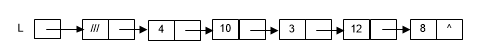
\includegraphics[scale=0.6]{images/SingleList.png}
		\caption{单个链表结构}
	\end{figure}
	其次设计多表管理系统的结构,其结构域中包含指向第一张表的指针start,指向最后一张表
	的指针end以及表的数量length。\par
	为了使管理系统更干净方便地管理链表,我把单张表的各种操作封装在一个类LinkList中,
	该类的域中包含指向空表头的指针head,指向表尾的指针tail和表长length,同时使用一个
	指针down指向该链表的下一张。该类起着连接单表和管理系统的作用(即通过十字链表进行存
	储)。\par
	\begin{figure}[H]
		\centering
		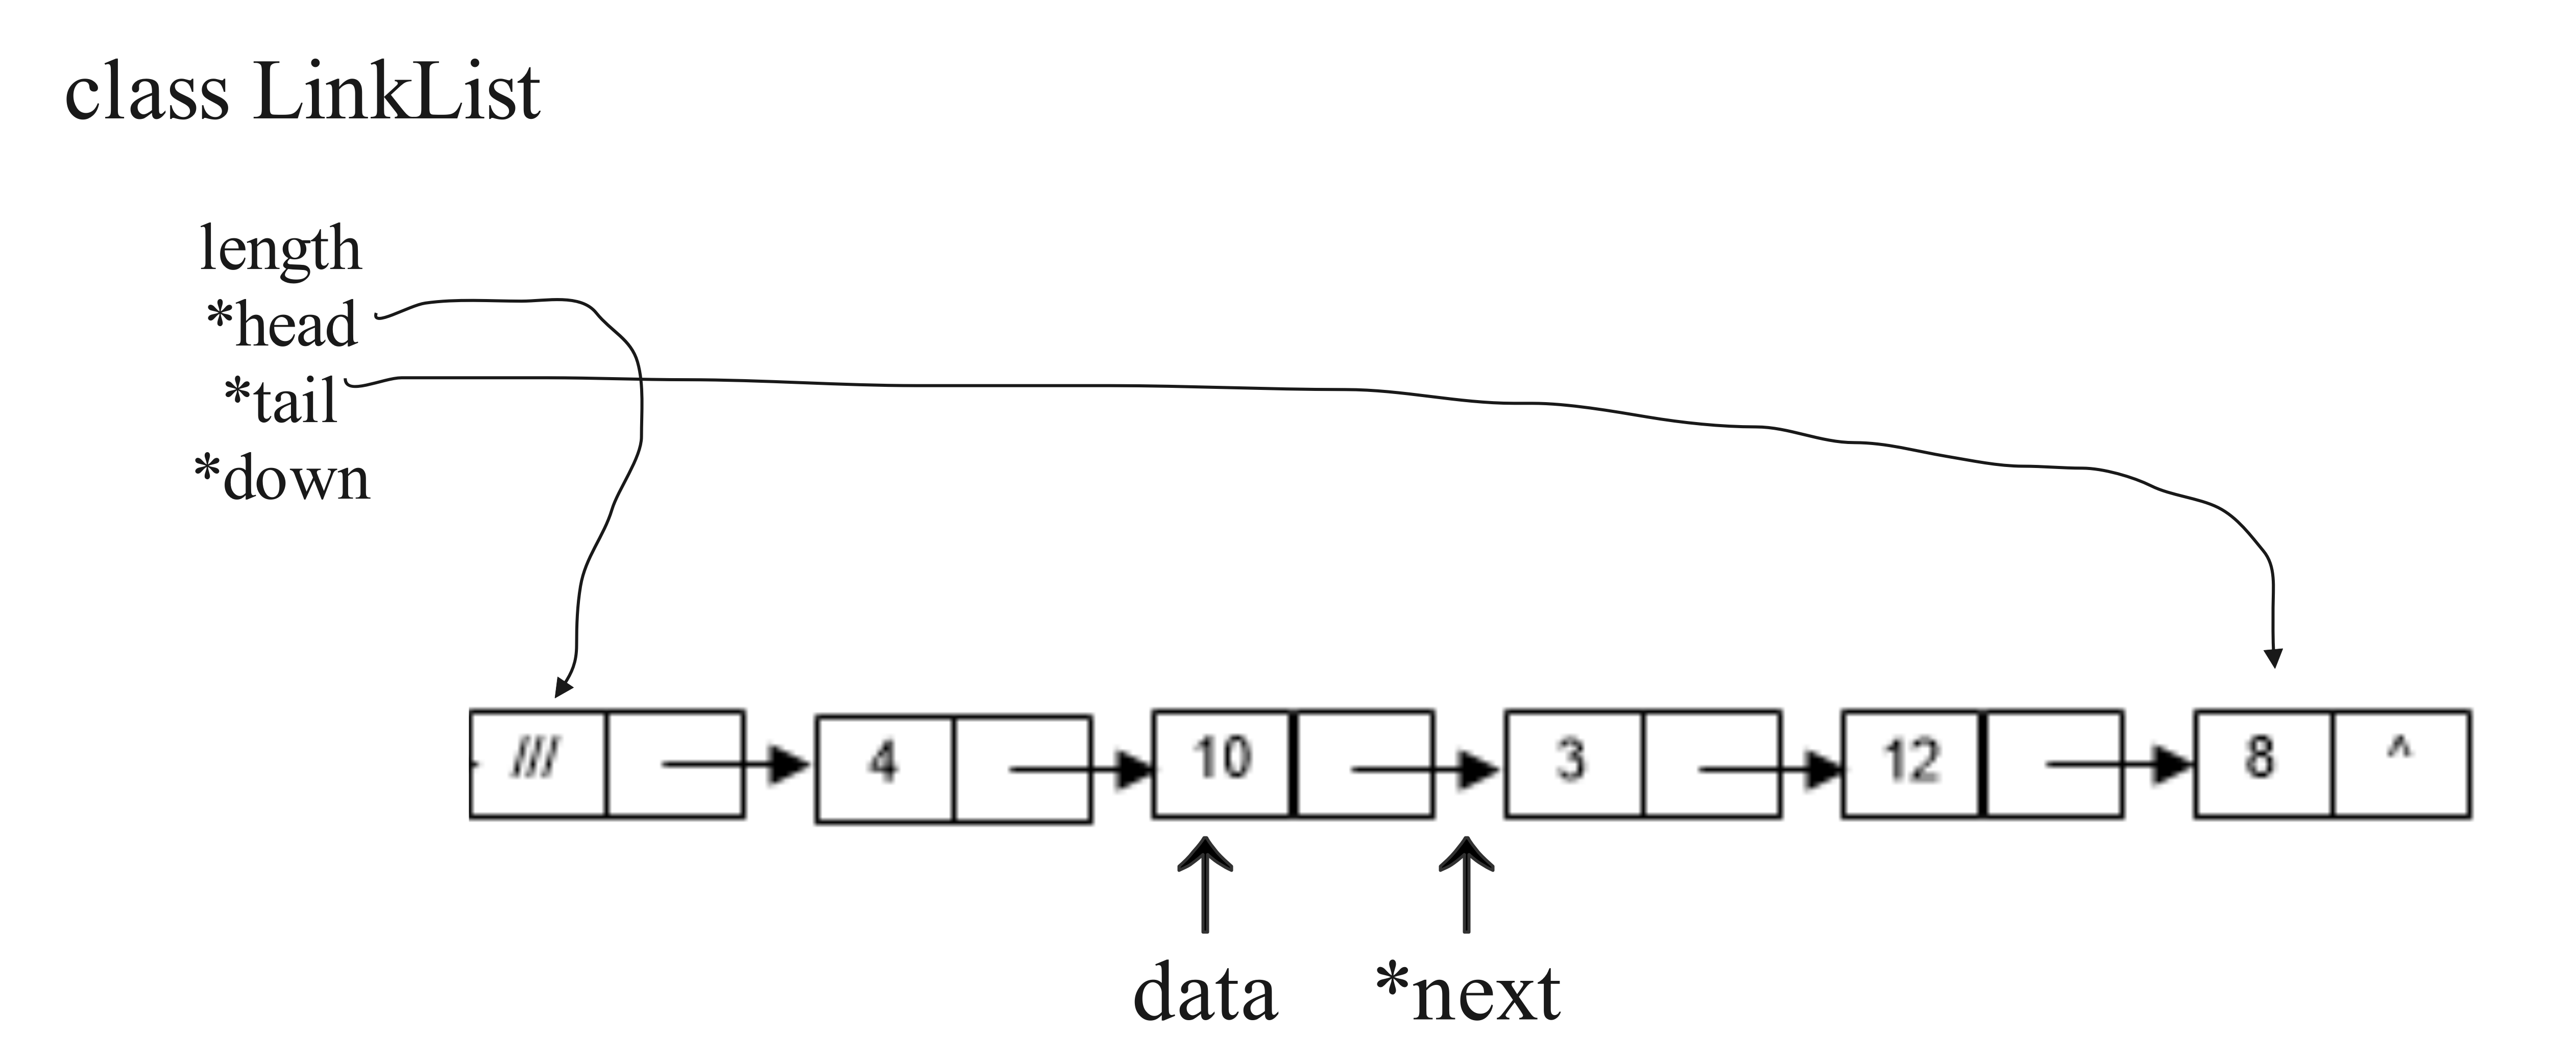
\includegraphics[scale=0.5]{images/LinkList.png}
		\caption{LinkList}
	\end{figure}
	\begin{figure}[H]
		\centering
		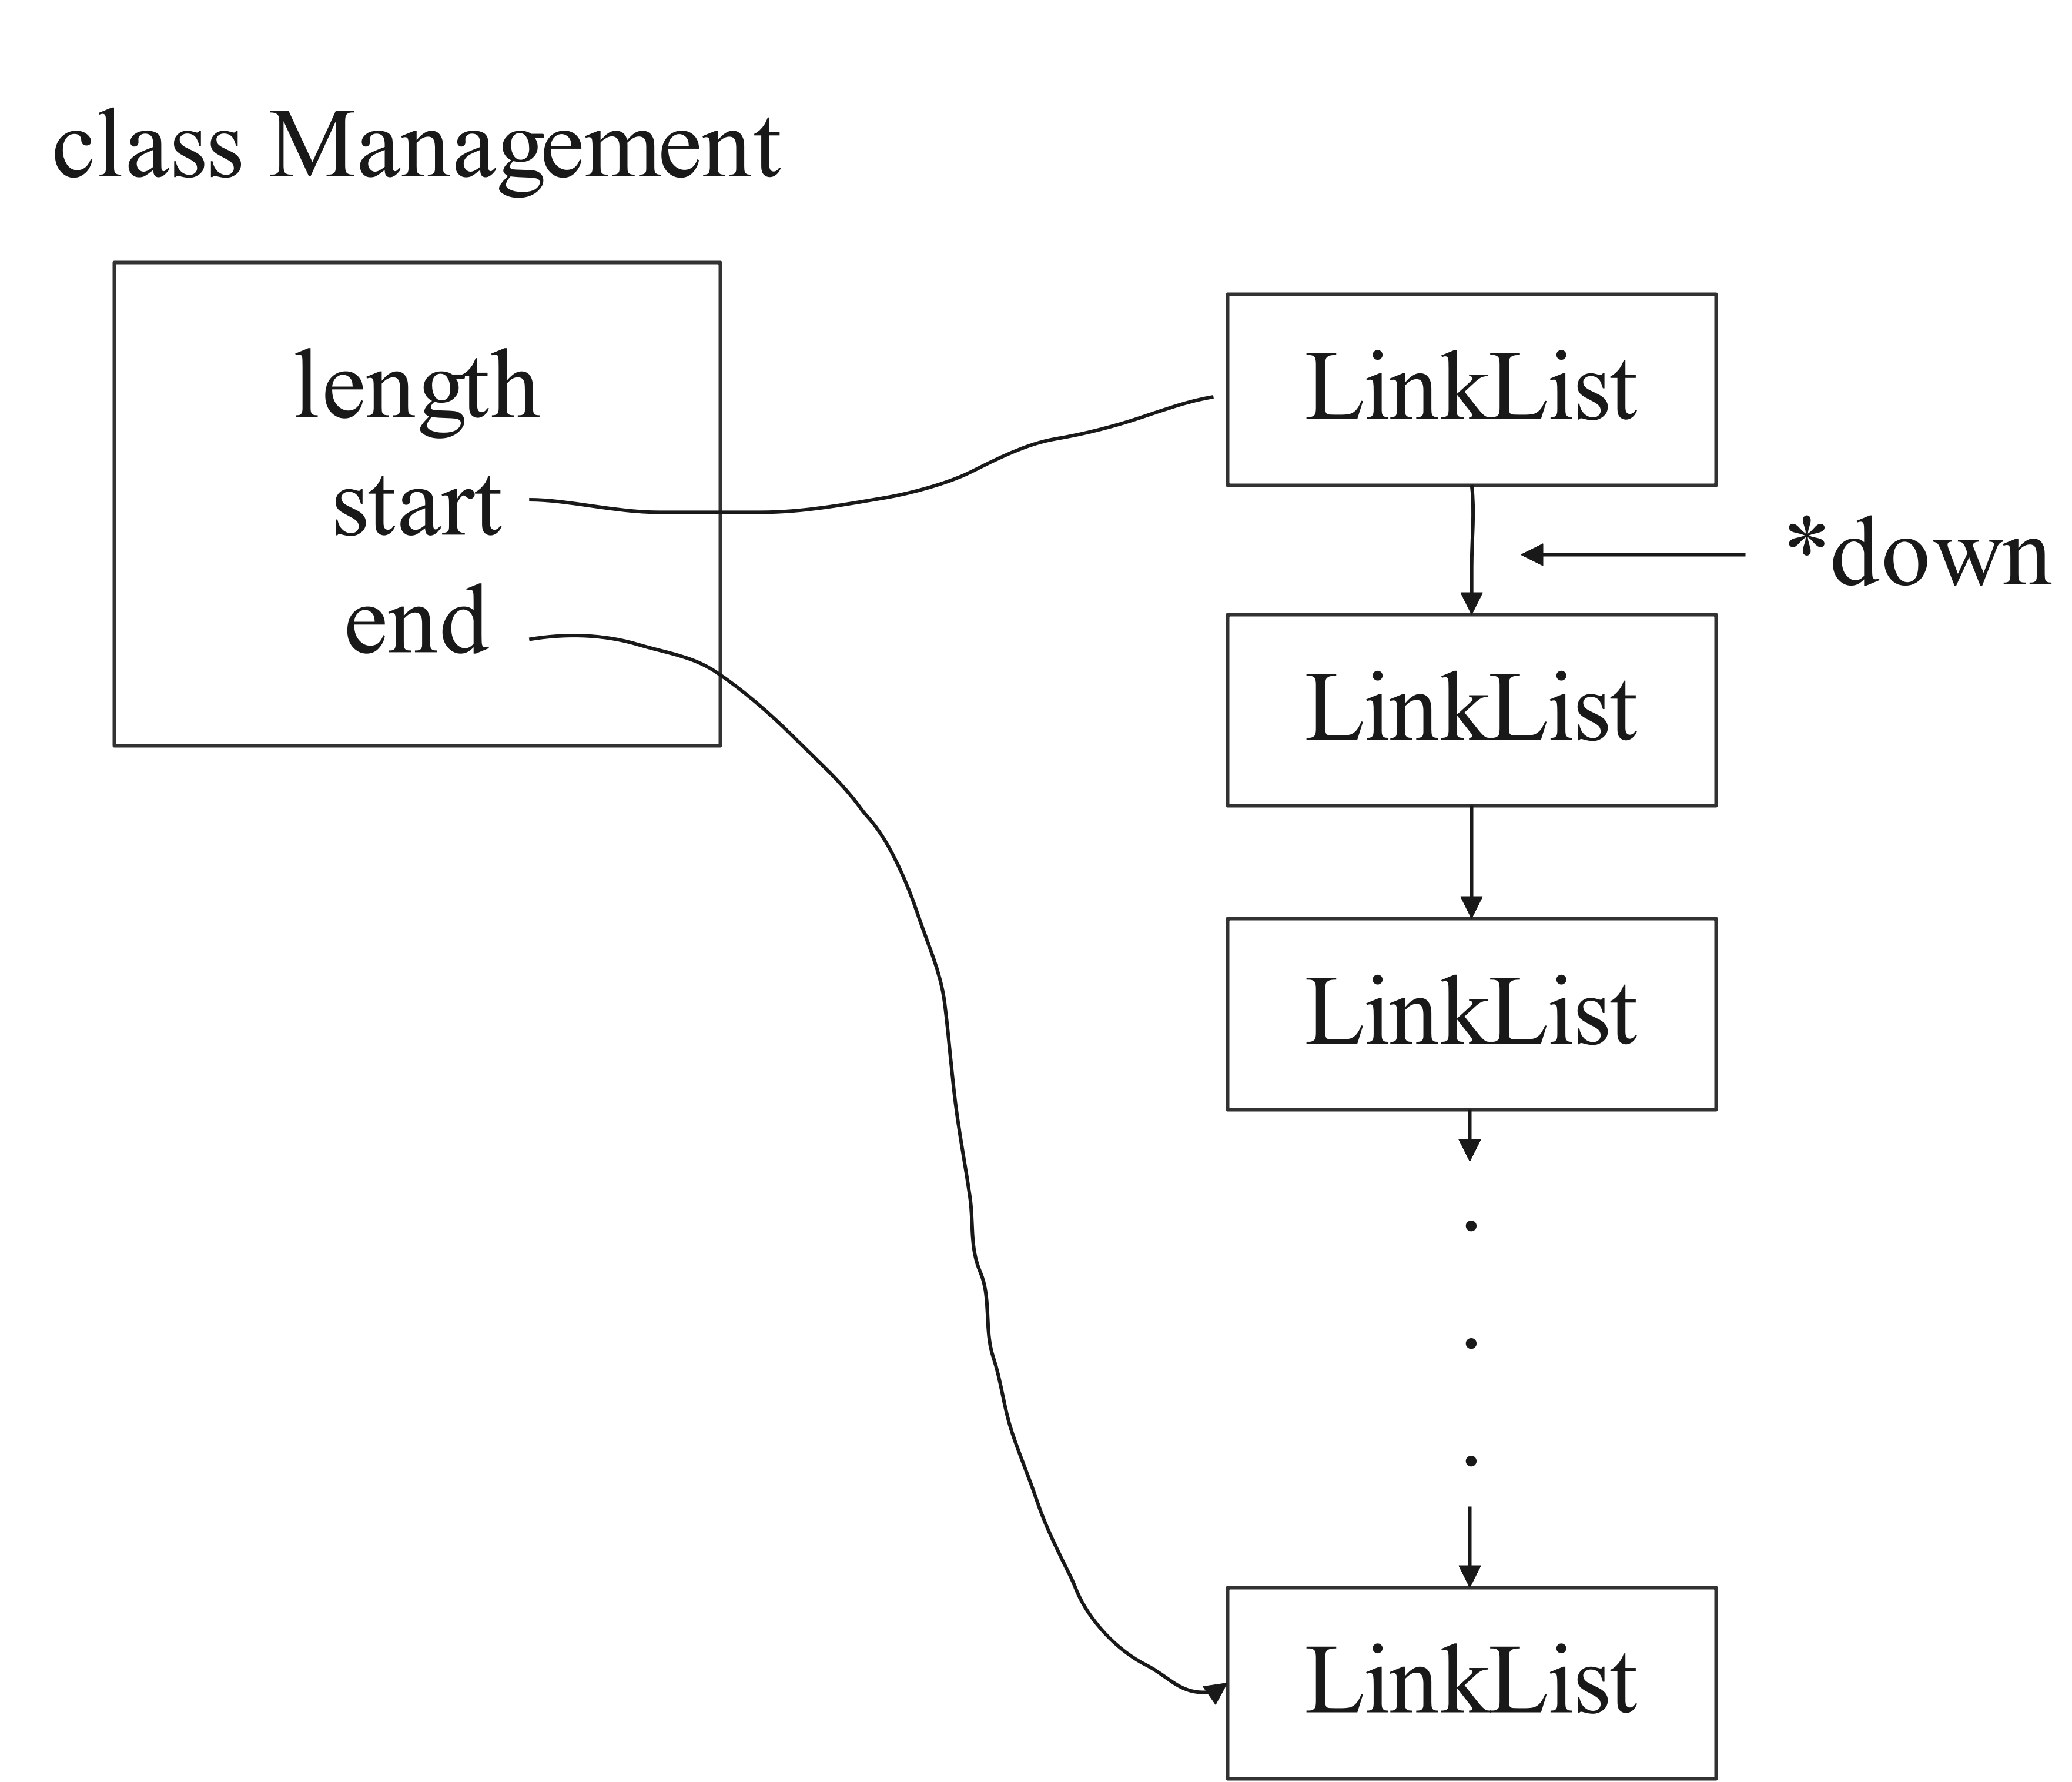
\includegraphics[scale=0.4]{images/Management.png}
		\caption{Management}
	\end{figure}
	\textbf{整体系统结构设计:}\par
	整个系统分为两层。\par
	最外层是管理系统Management,负责新增表、删除表、进入某个表进行操作(在这一层中,所
	有对单张表进行的操作都是杯被隐封装着的,
	只能通过接口single\_list\_op()进行访问)。\par
	内层是对单张表的操作,需要先进入一张表然后操作。随时可以返回管理系统进行其他操作
	。

\subsection{系统实现}
	\noindent \textbf{单表操作:}\par
	\begin{enumerate}
		\item InitList(L): 用malloc函数为链表分配空间即可。注意判断链表是否已存在。
		\item DestroyList(L): 使用free函数将所有分配空间的节点依次释放即可。注意判
		空。
		\item ClearList(L): 用free函数释放除头节点的空间即可。注意判空。
		\item ListEmpty(L): 由于前面及时用域length记录表长,表长为0返回false反之返
		回true。注意判空。
		\item ListLength(L): 与5思路相同。
		\item GetElem(L,i,e): 遍历线性表查找元素即可。注意判空。
		\item LocateElem(L,i,e): 思路同6。
		\item PriorElem(L,cur\_e,pre\_e): 思路同6。
		\item NextElem(L,cur\_e,next\_e): 思路同6.
		\item ListInsert(L,i,e): 通过遍历找到位置后用malloc新分配一个节点空间即可。
		注意判空。
		\item ListDelete(L,i,e): 通过遍历找到位置后调整指针域,释放节点即可。注意判
		空。
		\item ListTraverse(L,visit()): 遍历一遍输出即可。
		\item reverseList(L): 
		\item RemoveNthFromEnd(L,n): 
		删除倒数第n个节点,就是删除整数第$ListLength-n+1$个节点。
		\item sortList(L): 这里可以用两种方法:一是新建一个数组把链表的信息放到数组
		中,借助数组进行排序,但这样会使用额外的空间。二是可以使用冒泡排序的交换指针
		域形式,单轮排序的形式如图。
		\begin{figure}[H]
			\centering
			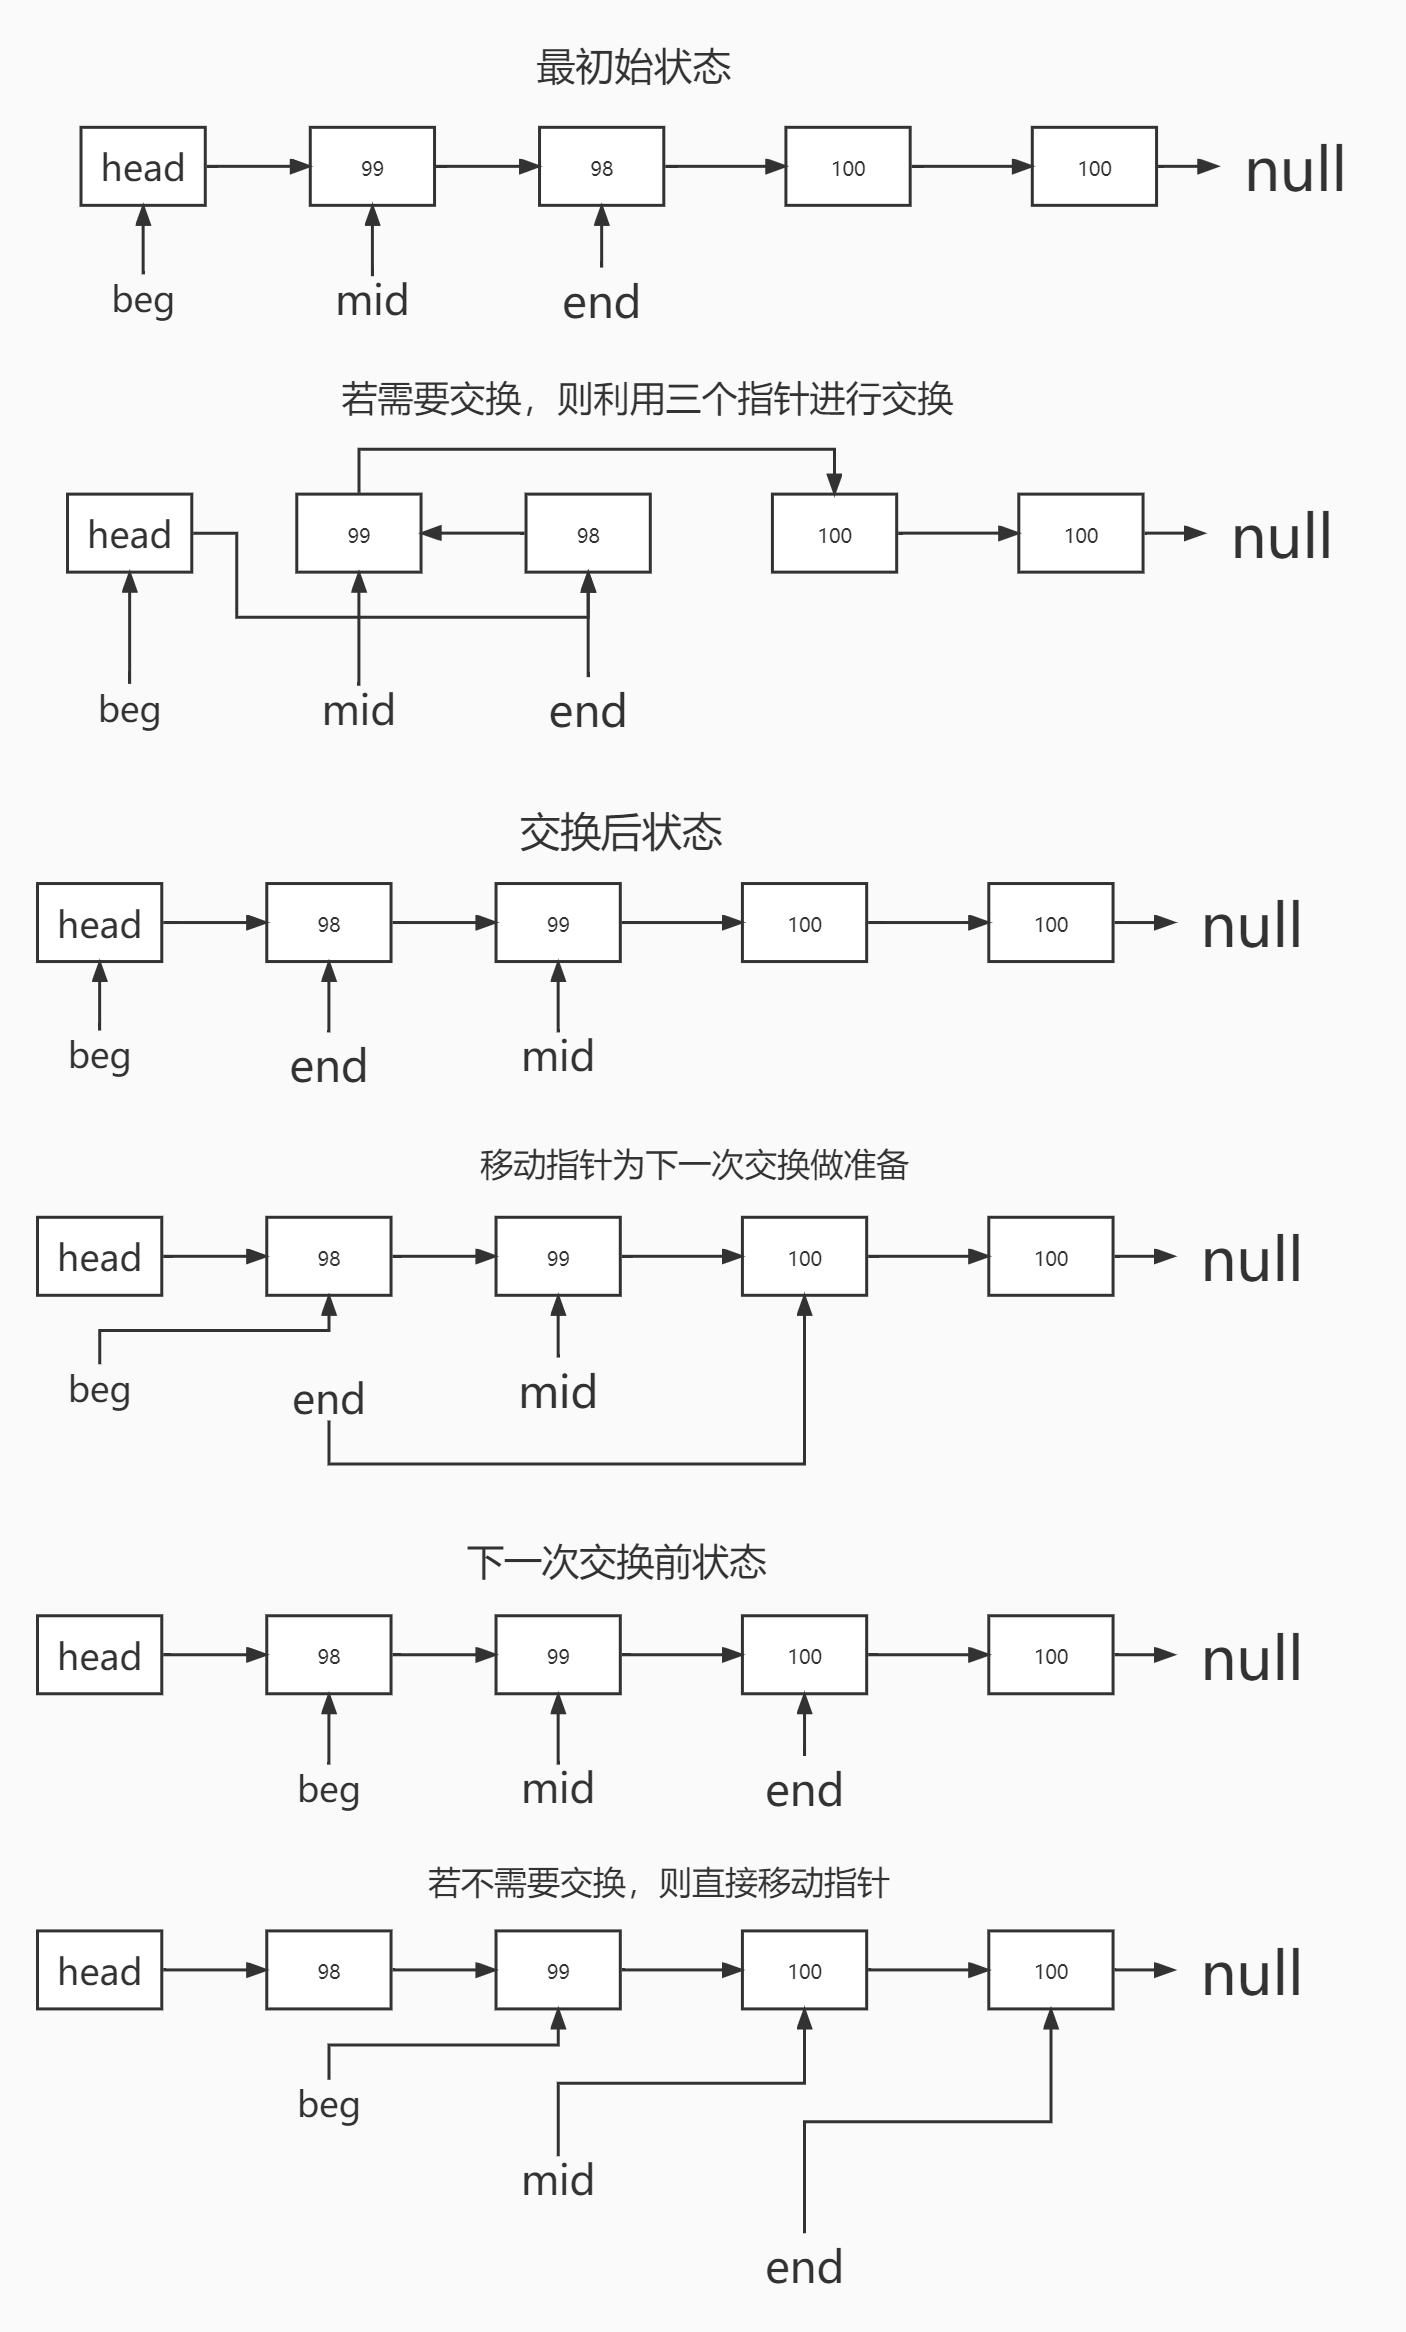
\includegraphics[scale=0.2]{images/链表排序.jpg}
			\caption{链表排序}
		\end{figure}
		\item SaveList(L,char FileName[]): 遍历一遍输出到文件流中即可。注意判空。
		\item LoadList(L,char FileName[]): 从文件流中读取数据,边读取便用malloc新
		建节点。注意判断线性表非空。
	\end{enumerate}
	\textbf{管理系统操作:}\par
	\begin{enumerate}
		\item NewList(): 在最后一张表down指针指向的位置为class 
		LinkList开辟空间即可,注意在构造函数中要将还没赋值的指针域置空。
		\item DelList(): 将指定位置的表空间全部释放,调节剩下的指针域即可。
	\end{enumerate}
	\textbf{一些自己写着玩的函数}
	\begin{enumerate}
		\item structure\_disp(Manager M): 用于展示管理系统展示树形目录。由于表的数
		目和层次结构比较简单,只需要用迭代来打印目录即可。打印存储情况及状态如图
		\begin{figure}[H]
			\centering
			\includegraphics[scale=0.3]{images/树形目录.bmp}
			\caption{打印树形目录}
		\end{figure}
	\end{enumerate}
	
\subsection{系统测试}
	\begin{enumerate}
		\item 新建一张线性表\par
		\TestTable{NewList}{1 2 -5 3 4 -7 -3 9 0}
		{创建成功并返回树形目录}{None}{None}
		实测结果:
		\InsertSingleFigure{images/链表测试结果/测试1-1}{0.5}{测试结果-1}
		\item 删除一张线性表\par
		\TestTable{DelList}{1}{删除成功并返回树形目录}{3}{index out of range!}
		实测结果:
		\InsertDoubleFigure{images/链表测试结果/测试2-1}
		{images/链表测试结果/测试2-2}{2}
		\item 销毁已存在的线性表\par
		\TestTable{DestroyList}{None}{销毁成功并返回树形目录}{None}{None}
		实测结果:
		\InsertSingleFigure{images/链表测试结果/测试3-1}{0.5}{测试结果-3}
		\item 清空线性表\par
		\TestTable{ClearList}{None}{清空成功并返回树形目录}{None(清空未初始化的表)}
		{显示表不存在}
		实测结果:
		\InsertDoubleFigure{images/链表测试结果/测试4-1}
		{images/链表测试结果/测试4-2}{4}
		\item 判断表是否为空\par
		\TestTable{ListEmpty}{None}{not empty!}{None(空表或者未初始化的表)}
		{显示empty list!}
		实测结果:
		\InsertDoubleFigure{images/链表测试结果/测试5-1}
		{images/链表测试结果/测试5-2}{5}
		\item 求表长\par
		\TestTable{ListLength}{None}{返回表长}{None(未初始化的表)}
		{显示empty list}
		实测结果:
		\InsertDoubleFigure{images/链表测试结果/测试6-1}
		{images/链表测试结果/测试6-2}{6}
		\item 获取指定位置元素\par
		\TestTable{GetElem}{元素位置}{返回对应元素}{元素位置(未初始化的表)}
		{显示empty list}
		实测结果:
		\InsertDoubleFigure{images/链表测试结果/测试7-1}
		{images/链表测试结果/测试7-2}{7}
		\item 获取元素位置\par
		\TestTable{LocateElem}{元素}{返回对应位置}{元素(不在表中)}
		{显示找不到元素}
		实测结果:
		\InsertDoubleFigure{images/链表测试结果/测试8-1}
		{images/链表测试结果/测试8-2}{8}
		\item 获取前驱\par
		\TestTable{PriorElem}{元素}{返回前驱}{元素(不在表中或无后继)}{显示找不到元
		素}
		实测结果:
		\InsertDoubleFigure{images/链表测试结果/测试9-1}
		{images/链表测试结果/测试9-2}{9}
		\item 获取后继\par
		\TestTable{NextElem}{元素}{返回前驱}{元素(不在表中或无后继)}{显示找不到元
			素}
		实测结果:
		\InsertDoubleFigure{images/链表测试结果/测试10-1}
		{images/链表测试结果/测试10-2}{10}
		\item 插入元素\par
		\TestTable{ListInsert}{2 11}{显示插入后遍历结果}{错误的插入位置}
		{显示位置错误}
		实测结果:
		\InsertDoubleFigure{images/链表测试结果/测试11-1}
		{images/链表测试结果/测试11-2}{11}
		\item 删除元素\par
		\TestTable{ListDelete}{2}{删除成功}{错误的删除位置}
		{显示位置错误}
		实测结果:
		\InsertDoubleFigure{images/链表测试结果/测试12-1}
		{images/链表测试结果/测试12-2}{12}
		\item 遍历表
		\TestTable{ListTraverse}{None}{遍历结果}{None}{None}
		实测结果:
		\InsertSingleFigure{images/链表测试结果/测试13-1}{0.7}{测试结果-13}
		\item 反转链表\par
		\TestTable{ListReverse}{None}{反转后遍历结果}{None}{None}
		实测结果:
		\InsertSingleFigure{images/链表测试结果/测试14-1}{0.7}{测试结果-14}
		\item 删除倒数第n个元素\par
		\TestTable{RemoveNthfromEnd}{1}{删除成功}{20}
		{显示位置错误}
		实测结果:
		\InsertDoubleFigure{images/链表测试结果/测试15-1}
		{images/链表测试结果/测试15-2}{15}
		\item 链表排序\par
		\TestTable{ListSort}{None}{排序后遍历结果}{None}{None}
		实测结果:
		\InsertSingleFigure{images/链表测试结果/测试16-1}{0.7}{测试结果-16}
		
	\end{enumerate}


\subsection{实验小结}
    \noindent \textbf{内容收获:}
    \begin{enumerate}
    	\item 掌握了链式结构存储的一些实现方式。基本任务圆满完成。
    	\item 复习了c++中类,STL,文件IO,友元函数等的基本用法。
    	\item 学习了如何使用VisualStudio + cmake搭建跨平台项目。
    \end{enumerate}
	\noindent \textbf{一些典型错误:}
	\begin{enumerate}
		\item 没有判断指针是否指向空导致segmentation fault。
		\item 文件忘记关闭,这在向文件输入时会导致文件是空的,输出时报错。
		\item 一个引用的问题:函数返回一个引用时要用引用来接受引用再进行操作。
	\end{enumerate}
	\noindent \textbf{经验:}
	\begin{enumerate}
		\item 头文件和源文件分离的结构,头文件中存放相关的函数、类声明,源文件中存放
		相关的定义。
		\item 对于一些小型课设,面向对象编程会造成一些不必要的冗余,还是使用面向过程
		编程更加方便(这也在二叉树的报告中体现了)。
		\item 能抽象成函数的部分尽量抽象成函数,重复的语句一定要用函数,否则后面调试
		维护时会很麻烦。
		\item 指针不用时一定要置空,并且使用指针时一定要判空。
	\end{enumerate}


\newpage

\section{基于二叉链表的二叉树实现}

\subsection{问题描述}
	为熟练掌握二叉树的各种基本运算,了解其逻辑结构与物理结构,我需要设计一个二叉树管
	理系统,实现二叉树的管理及其基本运算的实现(任务\ref{tasklist:2})。
	\begin{enumerate}\label{tasklist:2}
		\item 
		创建二叉树:函数名称是CreateBiTree(T,definition);初始条件是definition 给出
		二叉树T的定义,按照带空子树的二叉树前序遍历序列;操作结果是按definition构造
		二叉树T
		\item 
		销毁二叉树:函数名称是DestroyBiTree(T);初始条件是二叉树T已存在;操作结果是
		销毁二叉树T
		\item 清空二叉树:函数名称是ClearBiTree (T);初始条件是二叉树T存在;操作结果
		是将二叉树T清空
		\item 判定空二叉树:函数名称是BiTreeEmpty(T);初始条件是二叉树T存在;操作结
		果是若T为空二叉树则返回TRUE,否则返回FALSE
		\item 求二叉树深度:函数名称是BiTreeDepth(T);初始条件是二叉树T存在;操作结
		果是返回T的深度
		\item 查找结点:函数名称是LocateNode(T,e);初始条件是二叉树T已存在,e是和T
		中结点关键字类型相同的给定值;操作结果是返回查找到的结点指针,如无关键字为e的
		结点,返回NULL
		\item 
		结点赋值:函数名称是Assign(T,e,value);初始条件是二叉树T已存在,e是和T中结点
		关键字类型相同的给定值;操作结果是关键字为e的结点赋值为value
		\item 
		获得兄弟结点:函数名称是GetSibling(T,e);初始条件是二叉树T存在,e是和T中结点
		关键字类型相同的给定值;操作结果是返回关键字为e的结点的(左或右)兄弟结点指针。
		若关键字为e的结点无兄弟,则返回NULL
		\item 插入结点:函数名称是InsertNode(T,e,LR,c);初始条件是二叉树T存在,e是
		和T中结点关键字类型相同的给定值,LR为0或1,c是待插入结点;操作结果是根据LR为0
		或者1,插入结点c到T中,作为关键字为e的结点的左或右孩子结点,结点e的原有左子树
		或右子树则为结点c的右子树。特殊情况:c插入作为根结点?可以考虑LR为-1时,作为
		根结点插入,原根结点作为c的右子树。
		\item 删除结点:函数名称是DeleteNode(T,e);初始条件是二叉树T存在,e是和T中
		结点关键字类型相同的给定值。操作结果是删除T中关键字为e的结点;同时,如果关键
		字为e的结点度为0,删除即可;如关键字为e的结点度为1,用关键字为e的结点孩子代替
		被删除的e位置;如关键字为e的结点度为2,用e的左孩子代替被删除的e位置,e的右子
		树作为e的左子树中最右结点的右子树
		\item 
		前序遍历:函数名称是PreOrderTraverse(T,Visit());初始条件是二叉树T存在,Visit
		是一个函数指针的形参(可使用该函数对结点操作);操作结果:先序遍历,对每个结点
		调用函数Visit一次且一次,一旦调用失败,则操作失败。
		\item 
		中序遍历:函数名称是InOrderTraverse(T,Visit));初始条件是二叉树T存在,Visit
		是一个函数指针的形参(可使用该函数对结点操作);操作结果是中序遍历t,对每个结点
		调用函数Visit一次且一次,一旦调用失败,则操作失败
		\item 后序遍历:函数名称是PostOrderTraverse(T,Visit));初始条件是二叉树T存
		在,Visit是一个函数指针的形参(可使用该函数对结点操作);操作结果是后序遍历t,
		对每个结点调用函数Visit一次且一次,一旦调用失败,则操作失败
		\item 按层遍历:函数名称是LevelOrderTraverse(T,Visit));初始条件是二叉树T存
		在,Visit是对结点操作的应用函数;操作结果是层序遍历t,对每个结点调用函数Visit
		一次且一次,一旦调用失败,则操作失败
		\item 
		最大路径和:函数名称是MaxPathSum(T),初始条件是二叉树T存在;操作结果是返回根
		节点到叶子结点的最大路径和
		\item 最近公共祖先:函数名称是LowestCommonAncestor(T,e1,e2);初始条件是二叉
		树T存在;操作结果是该二叉树中e1节点和e2节点的最近公共祖先
		\item 函数名称是InvertTree(T),初始条件是线性表L已存在;操作结果是将T翻转,
		使其所有节点的左右节点互换
		\item 实现线性表的文件形式保存:其中,(1)需要设计文件数据记录格式,以高效保存
		二叉树数据逻辑结构(D,{R})的完整信息;(2)需要设计二叉树文件保存和加载操作合理
		模式
		\item 实现多个二叉树管理:可采用线性表的方式管理多个二叉树,线性表中的每个数
		据元素为一个二叉树的基本属性,至少应包含有二叉树的名称。基于顺序表实现的二叉
		树管理
	\end{enumerate}

\subsection{系统设计}
	\noindent \textbf{数据结构设计:}\par
	首先是一棵二叉树的设计,通过二叉链表的方式实现,每个节点有指向孩子的指针*lchild,
	*rchild和节点的信息域data。
	\begin{figure}[H]
		\centering
		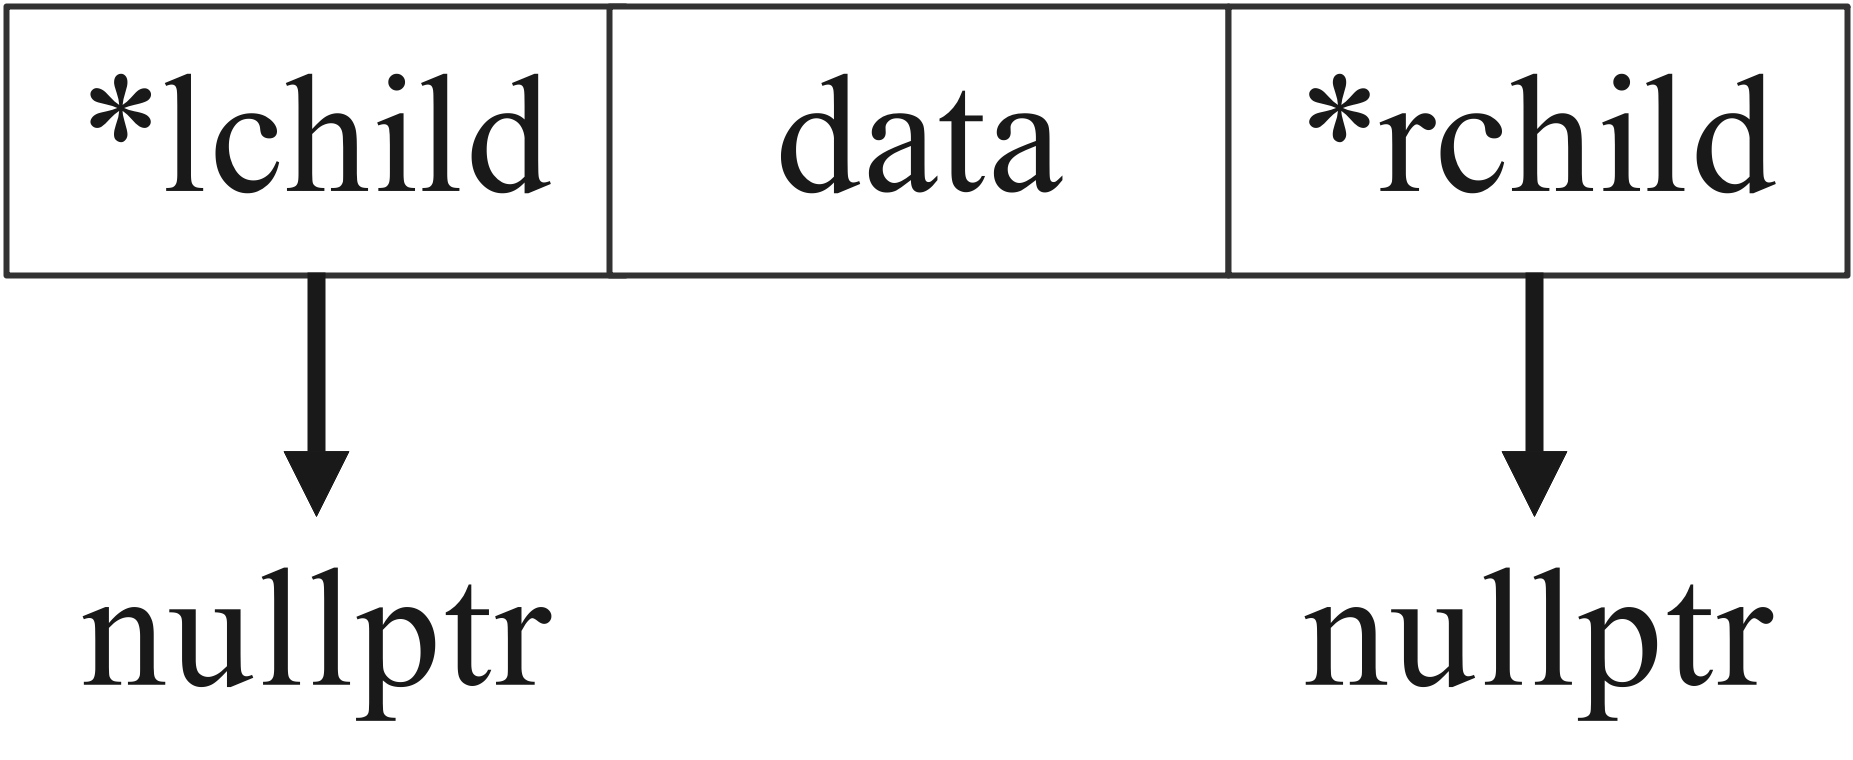
\includegraphics{images/单个二叉树节点.png}
		\caption{单个二叉树节点}
	\end{figure}
	其次是管理系统的设计,为方便,使用一个数组来线性存储二叉树。该数组与域size
	、length共同组成一个类Manager。同时,为了便于操作,我为每棵二叉树分配了一个
	name域来标识二叉树。\par
	整体结构如下:\par
	\begin{figure}[H]
		\centering
		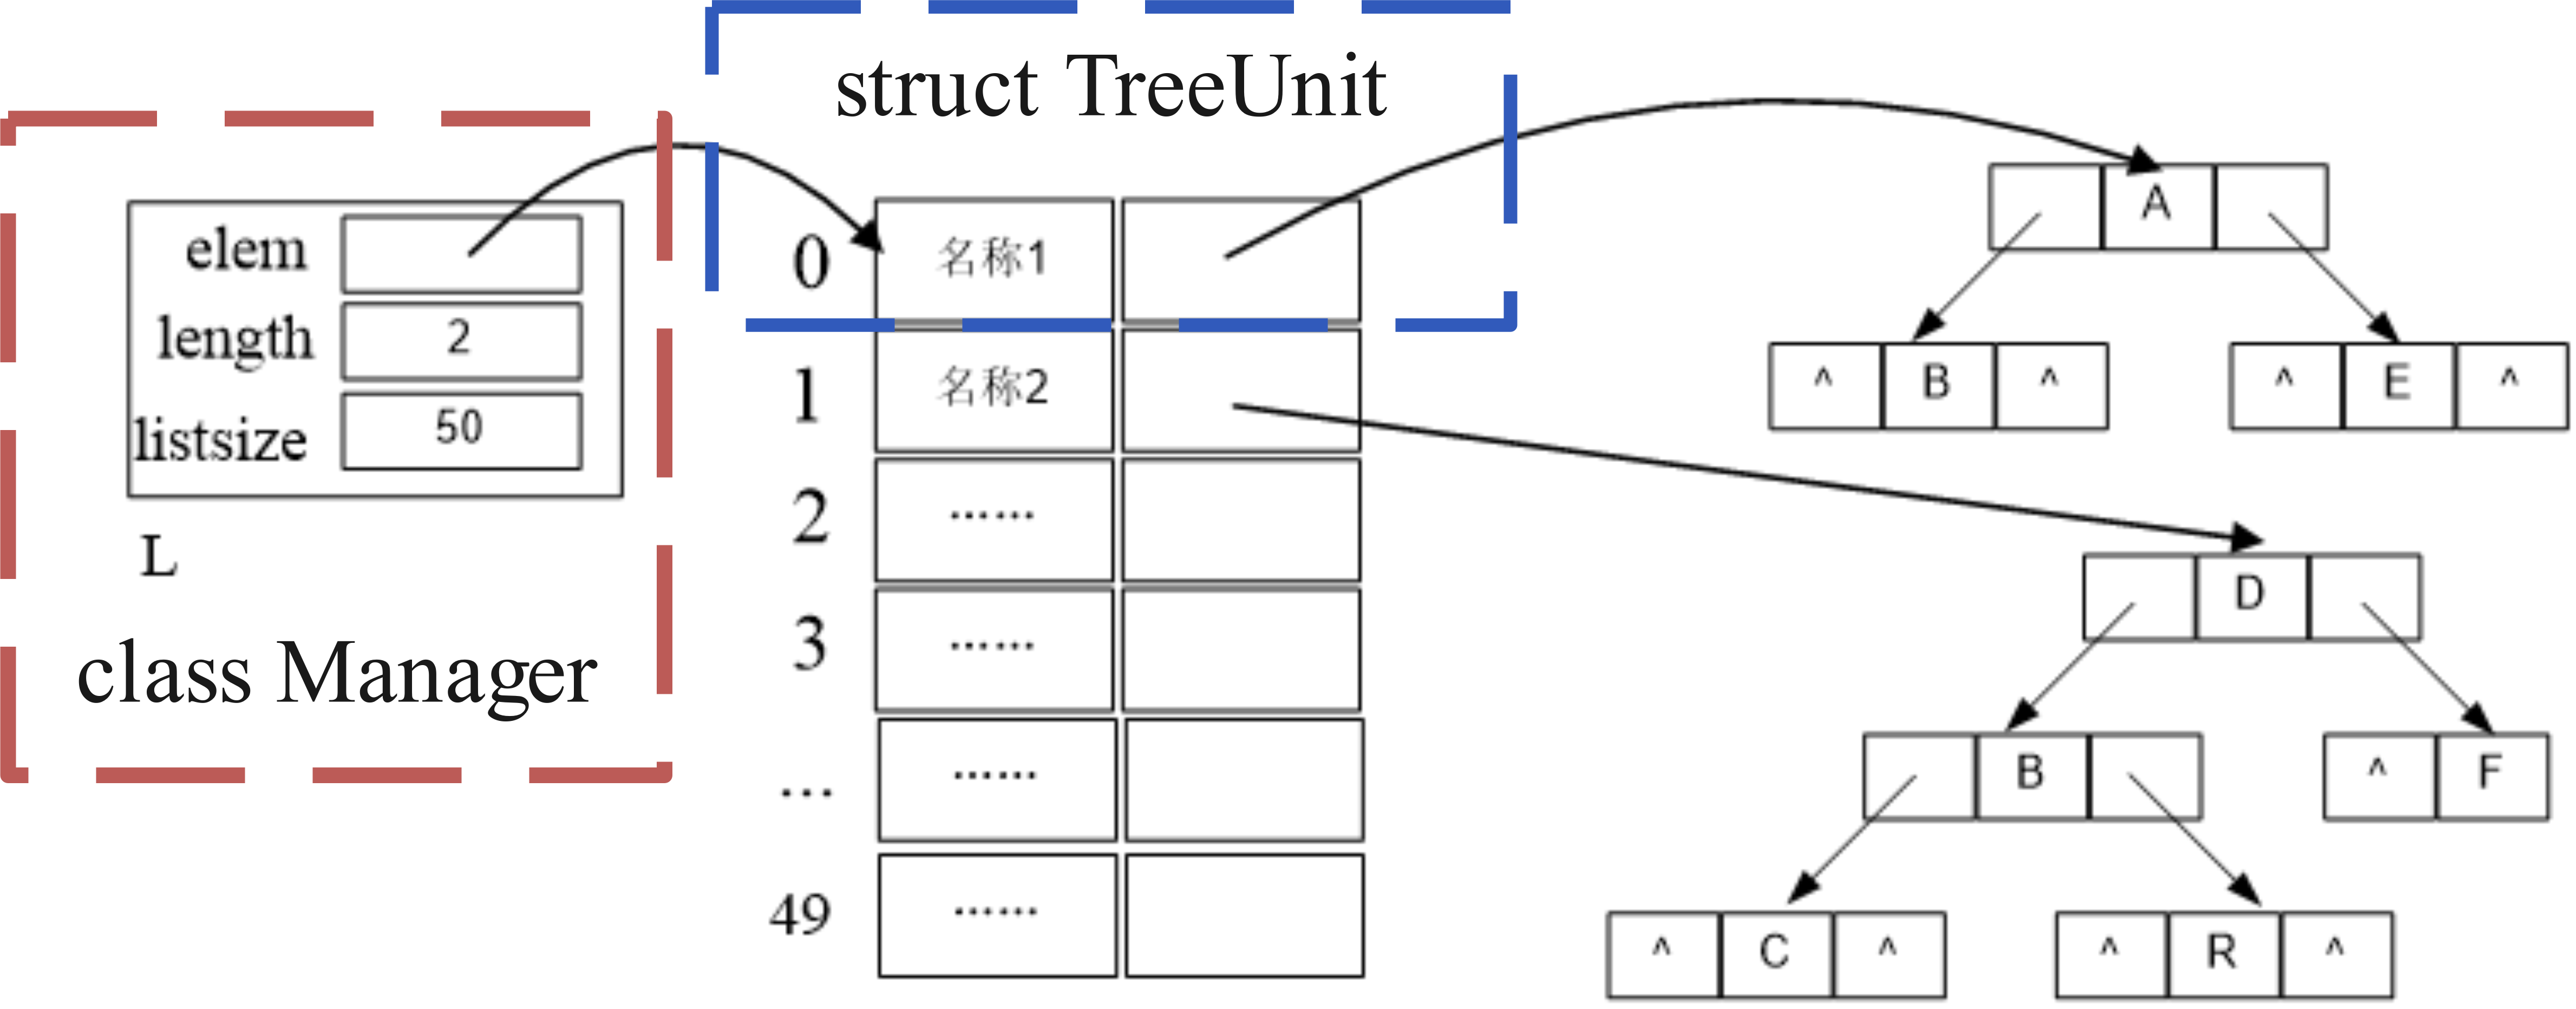
\includegraphics[scale=0.7]{images/二叉树管理系统结构.png}
		\caption{整体结构}
	\end{figure}
	\noindent \textbf{整体系统结构设计设计:}\par
	按照项目规范,依然使用多文件编译进行架构。其中,CMakeLists.txt是cmake构建文件;main.cpp
	文件用于获取外部命令并执行相应的函数;def.h存放引入的头文件、宏定义、以及结构体的
	定义;SingleTree模块存放单棵树相关操作的函数声明与定义;Manager模块存放类Manager
	。除了用类进行多棵二叉树的管理,程序主要采用面向过程编程的思想。
	\begin{figure}[H]
		\centering
		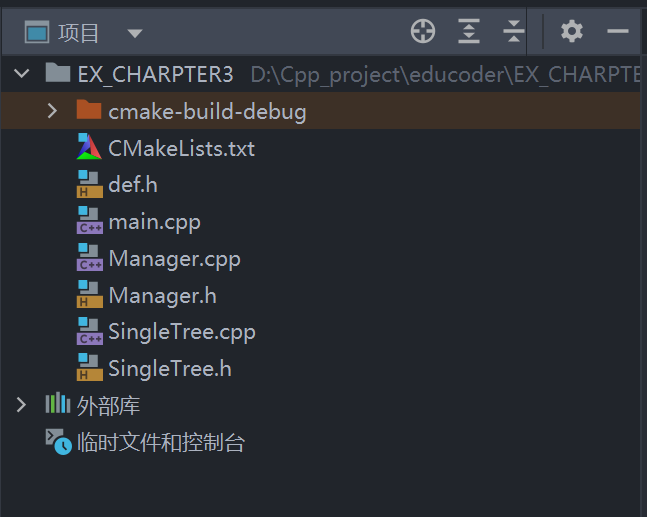
\includegraphics{images/二叉树程序架构.png}
		\caption{二叉树程序框架}
	\end{figure}

\subsection{系统实现}

	\noindent \textbf{单棵二叉树操作}
	\begin{enumerate}
		\item 创建二叉树:先用一个辅助函数GetData获取先序遍历数据(带空节点),然后使用
		一个递归函数build递归地、先序地构造一棵二叉树。
		\item 销毁二叉树:用后序遍历的思想,先回收左节点,再回收右节点,最后回收自身
		。注意递归终止条件是碰到空节点。
		\item 判空二叉树:判断传入的参数*T是否指向空即可。
		\item 
		求二叉树深度:用后序遍历的思想,自身节点的深度等于左右孩子的较大者加一,即表
		达式$depth_{cur} = max(depth_{lc},depth_{rc}) + 1$.
		\item 查找节点:用先序遍历思想,若自身不是则去找左右孩子。递归终止条件是节点
		为空。伪代码如下:
		\begin{shaded*}\begin{alg}{查找节点}
				\begin{algorithmic}
					\Input root of the tree: T
					\Output target tree node
					\Procedure{find}{$T$}
					\If $T$ is $nullptr$
					\State \Return $nullptr$
					\EndIf
					\If $T$ is the $target$
					\State \Return $T$
					\EndIf\par
					$l = find(T->lchild)$\par
					$r = find(T->rchild)$
					\State \Return $l$ or $r$ or $nullptr$ according to the 
					result
					\EndProcedure
				\end{algorithmic}
		\end{alg}\end{shaded*}
		\item 节点赋值:先找到节点,然后进行修改即可。
		\item 获得兄弟节点:用先序遍历思想,先判断自身的左右孩子是否满足条件,再递归
		地判断左右孩子。注意递归终止条件是节点为空。
		\item 插入节点:先找到插入位置,再用malloc分配一个新节点,调整原有的指针指向
		即可。
		\item 删除节点:对查找函数进行略微改动(大体框架变成了一个带返回值的递归,节点
		的修改关键就在于递归!),在查找到节点后进行指针域的调节,调节
		要分情况:\par
		第一种情况:要删除的节点是叶子节点:直接free后返回nullptr即可。
		如图\ref{delete:1}
		\begin{figure}[H]
			\centering
			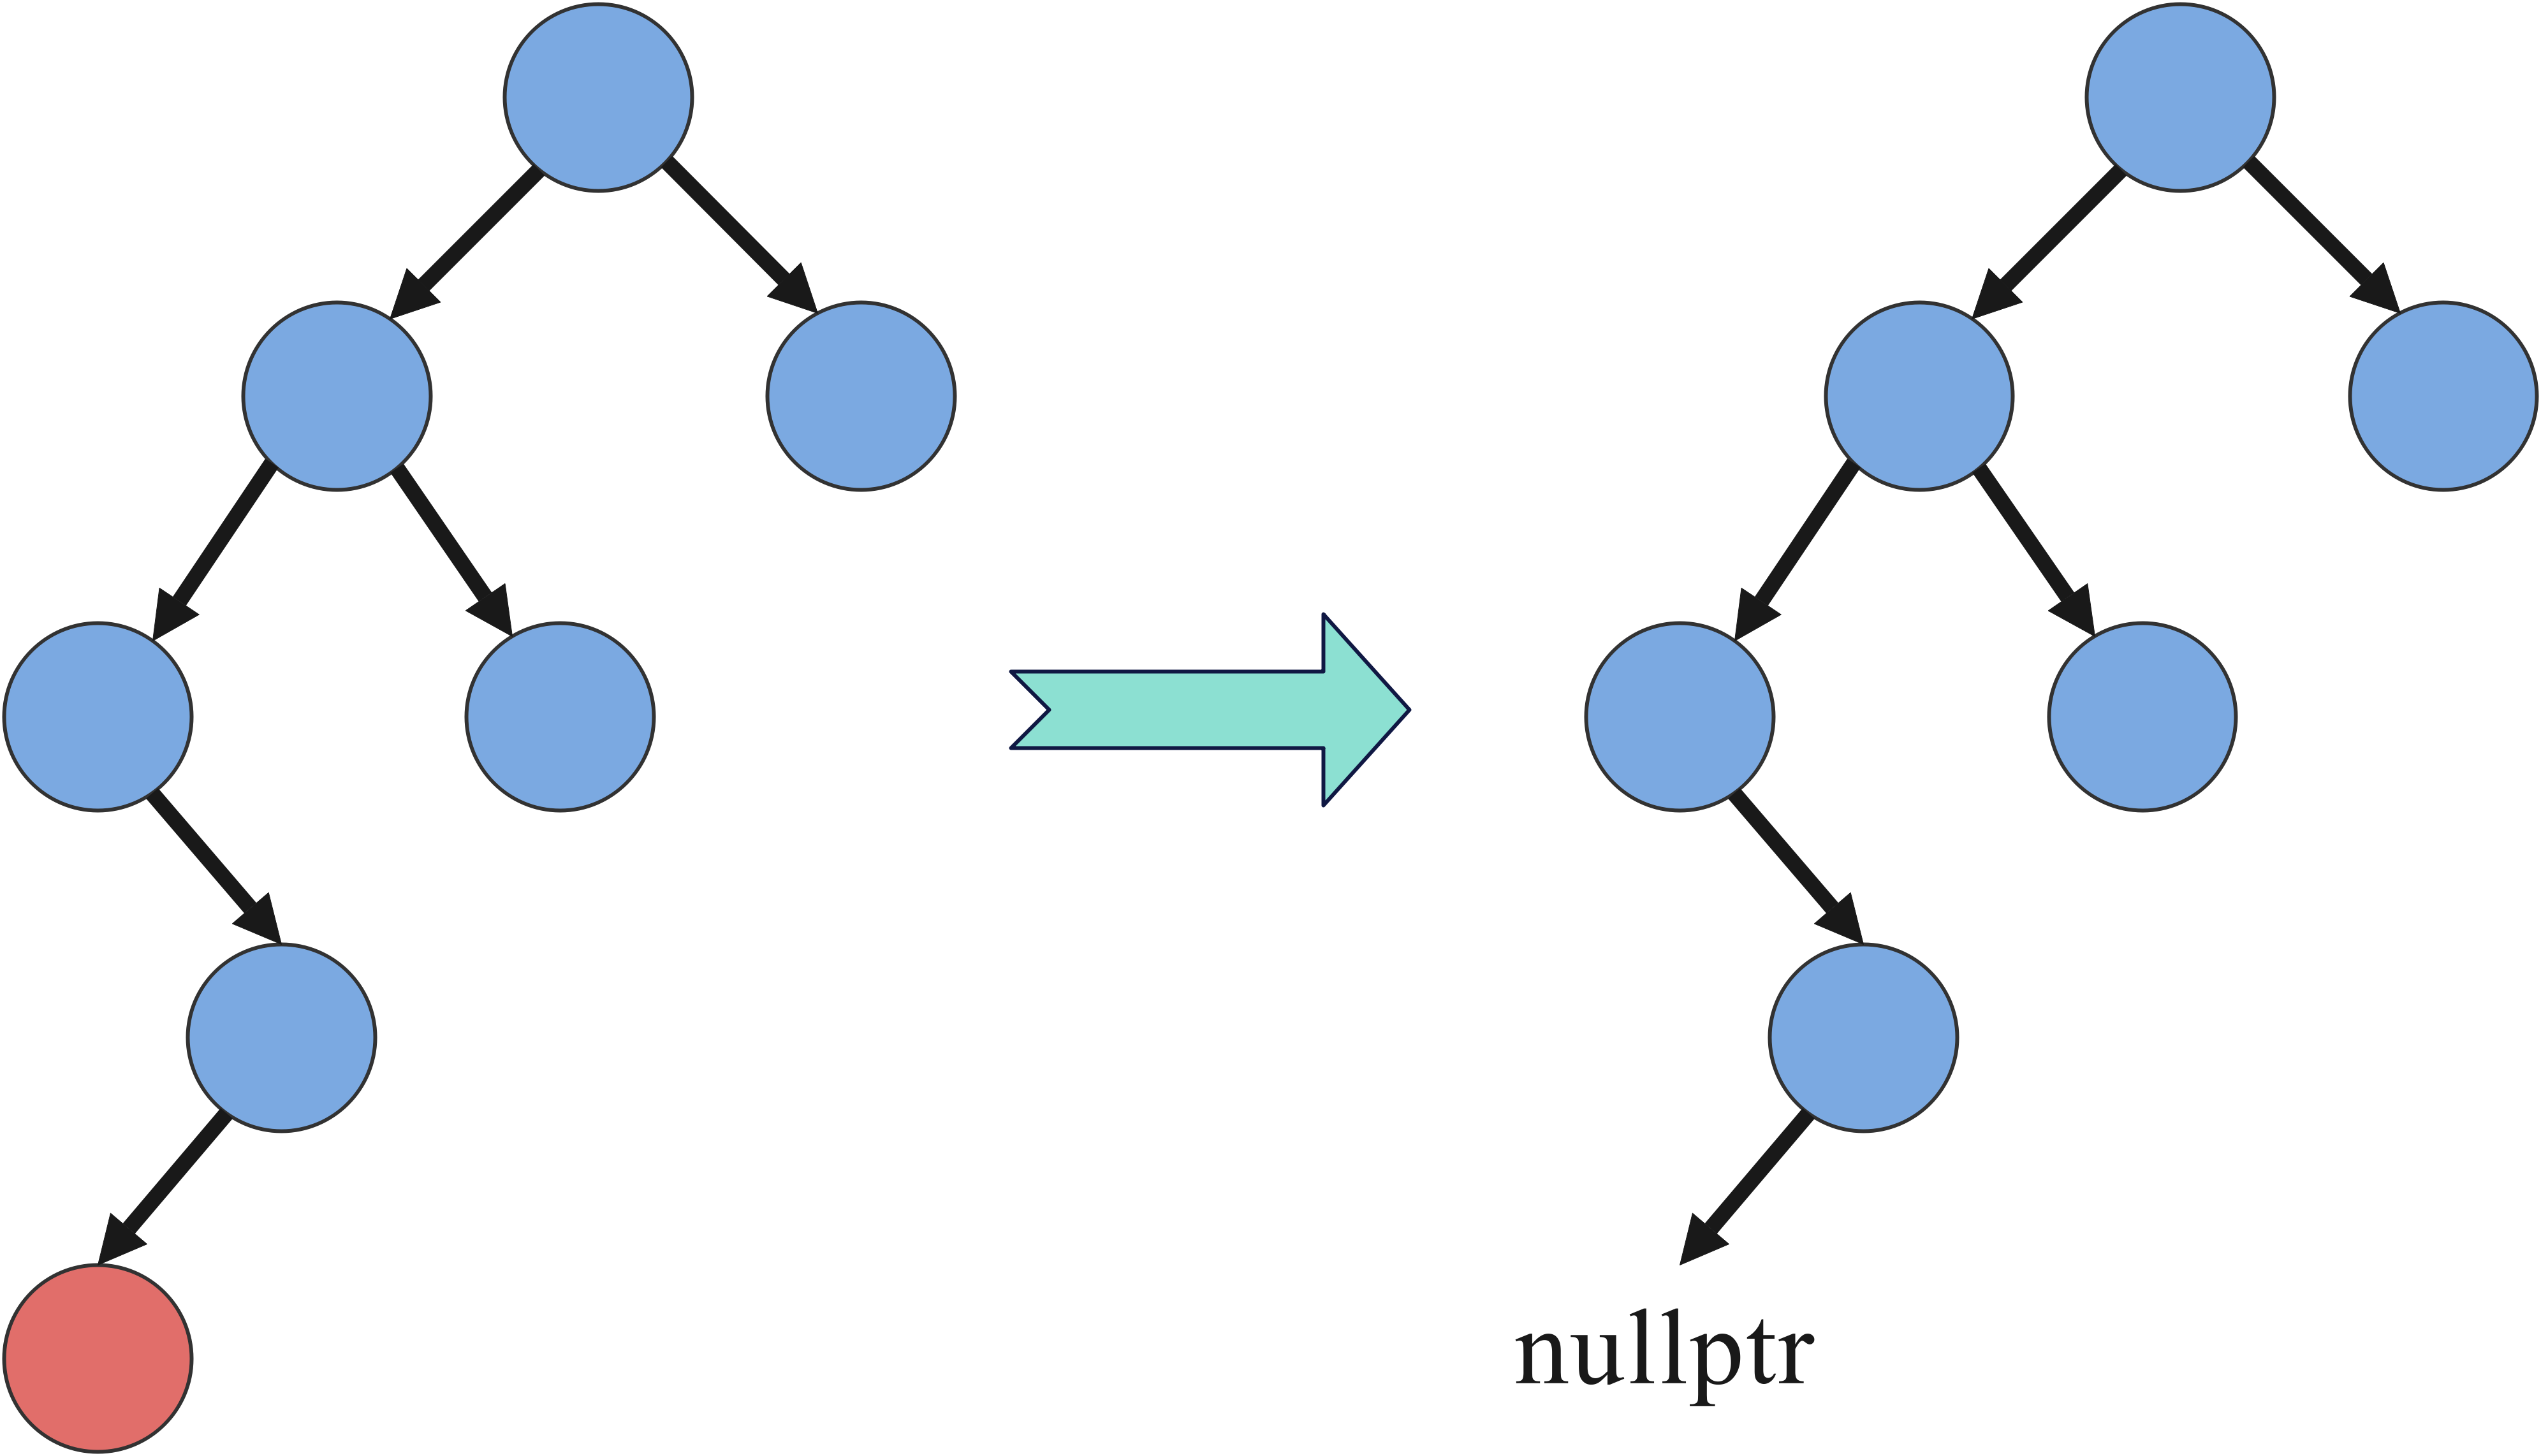
\includegraphics[scale=0.7]{images/二叉树删除节点1.png}
			\caption{删除节点-情况1}
			\label{delete:1}
		\end{figure}
		第二种情况:要删除的节点只有一个孩子节点:free当前节点,将此孩子节点返回即可
		。如图\ref{delete:2}
		\begin{figure}[H]
			\centering
			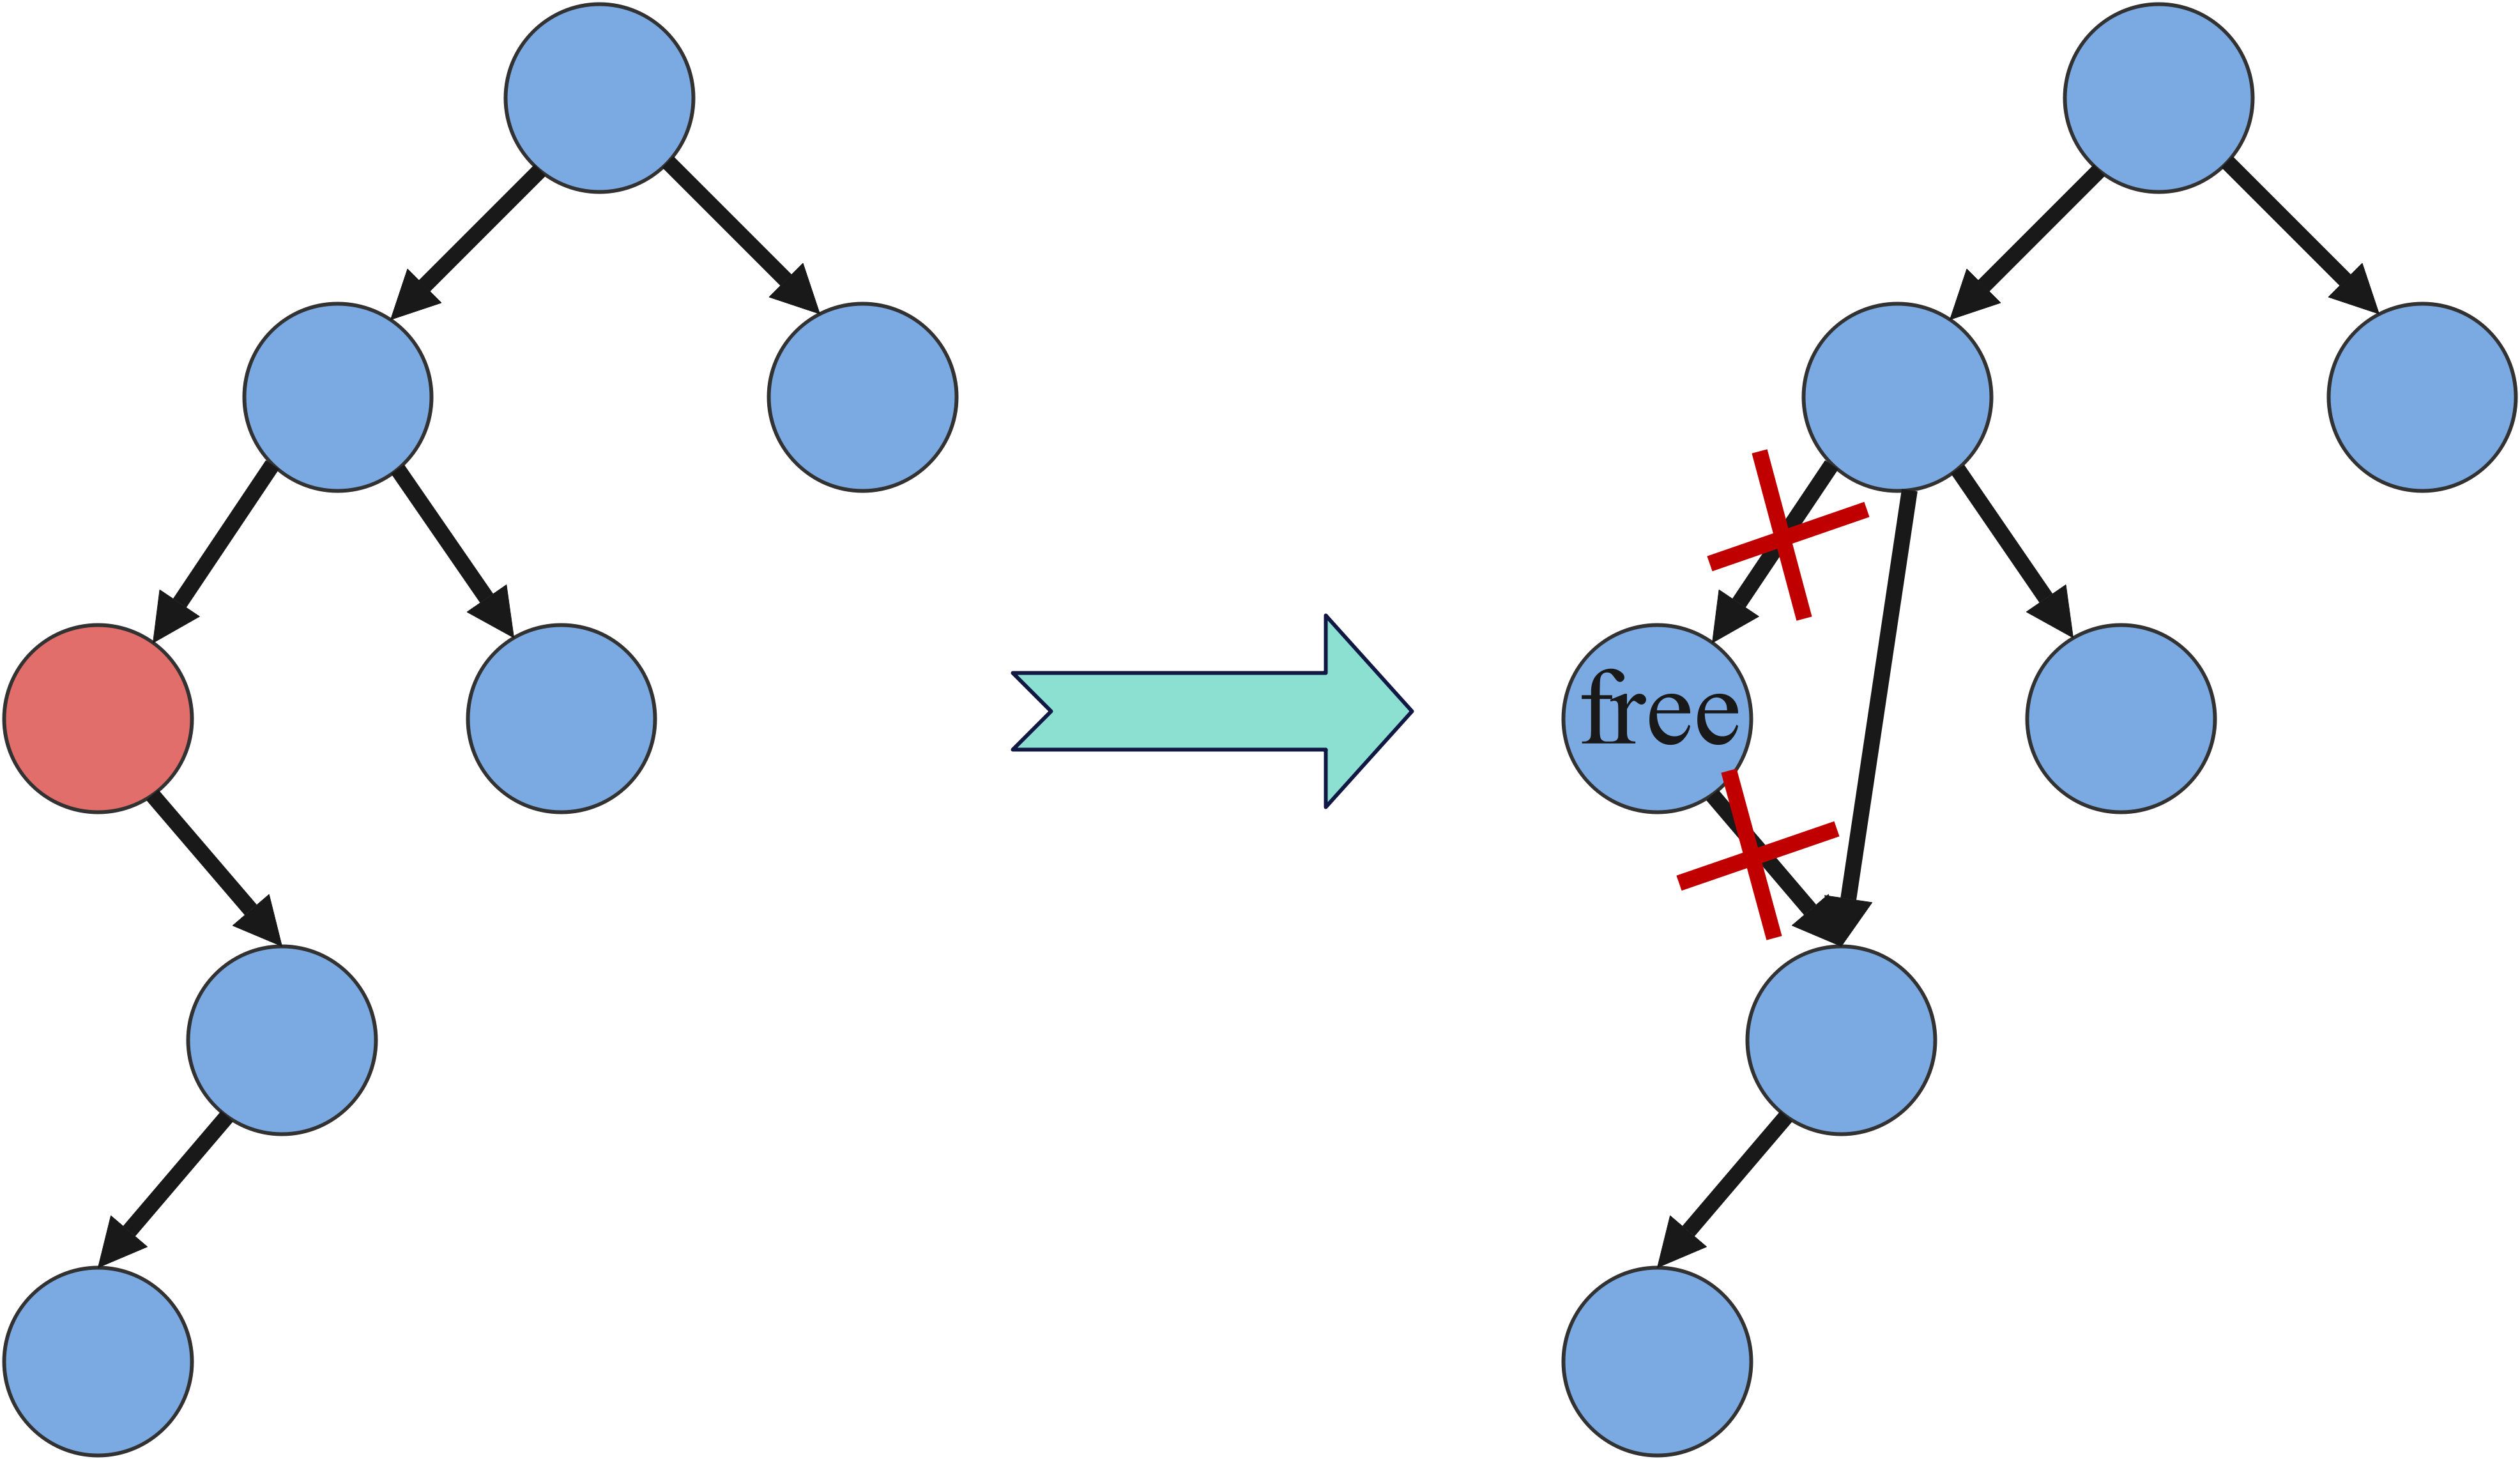
\includegraphics[scale=0.7]{images/二叉树删除节点2.png}
			\caption{删除节点-情况2}
			\label{delete:2}
		\end{figure}
		第三种情况:要删除的节点既有左孩子又有右孩子:将右子树挂到左子树的“最右侧”。
		如图\ref{delete:3}
		\begin{figure}[H]
			\centering
			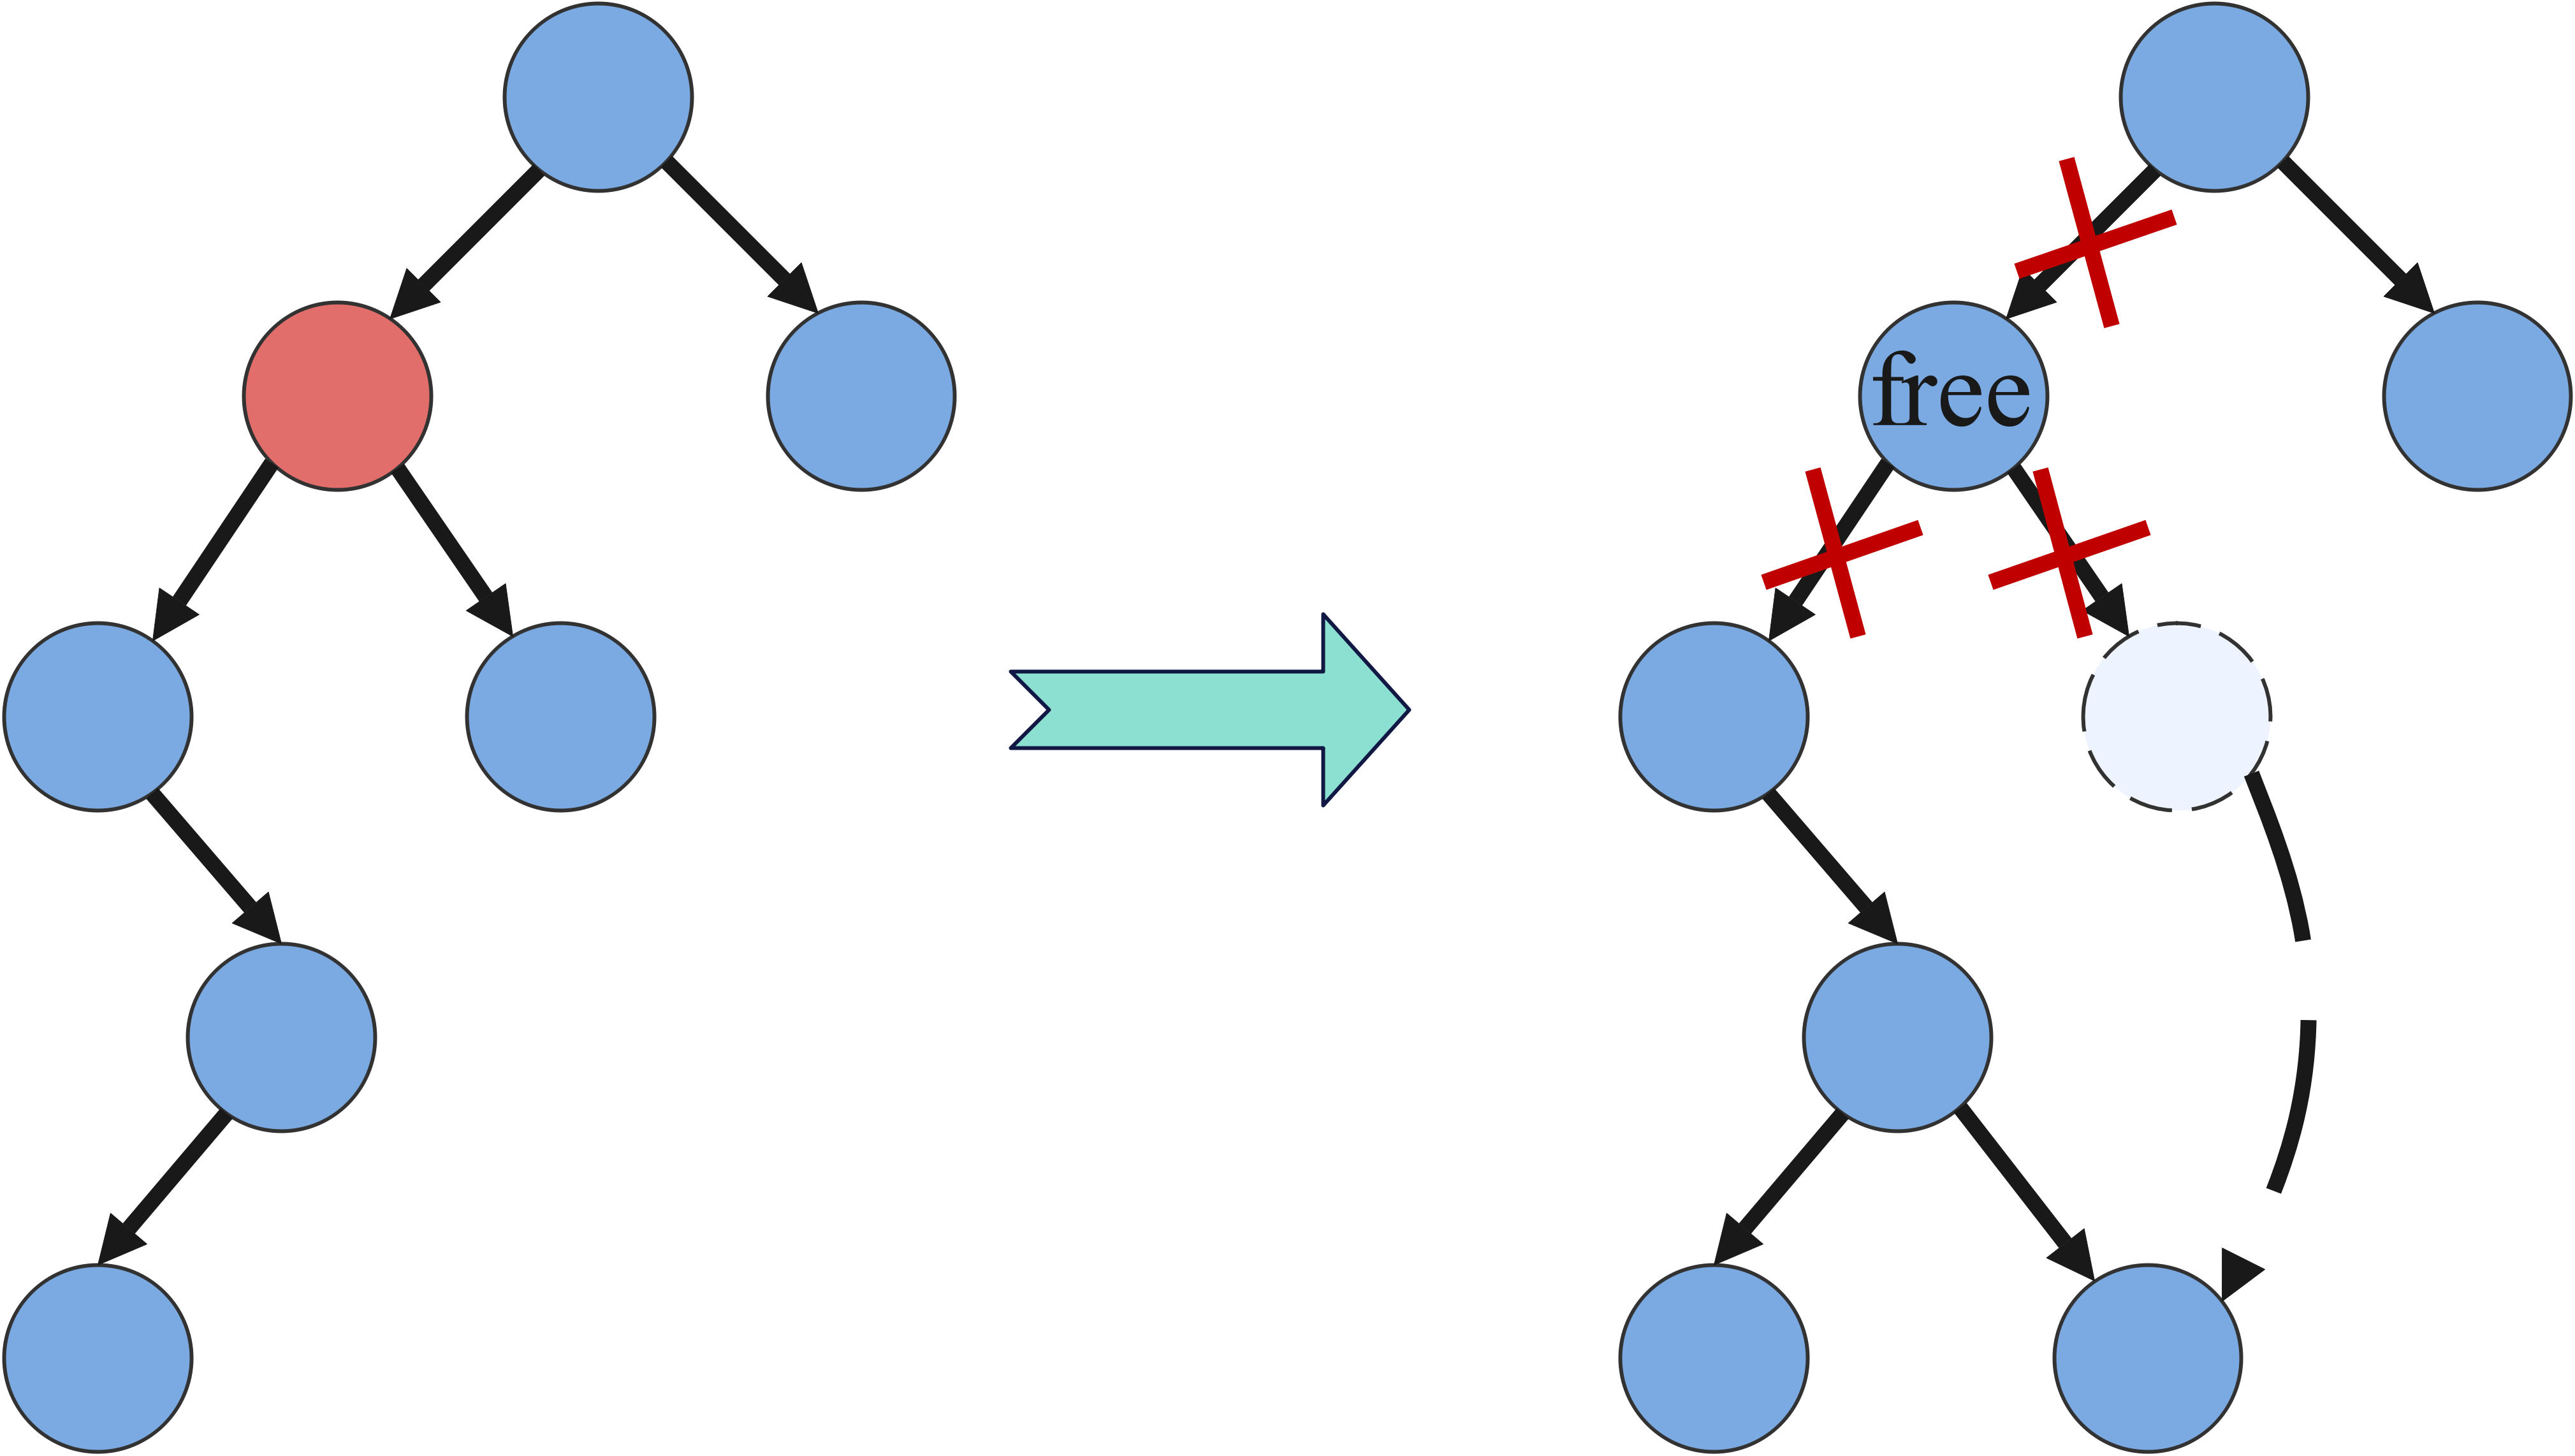
\includegraphics[scale=0.7]{images/二叉树删除节点3.png}
			\caption{删除节点-情况3}
			\label{delete:3}
		\end{figure}
		\item 前序遍历:这里采用非递归的方式实现。将节点按照中-右-左的顺序入栈,出栈
		时先访问,然后继续按照这样判断直到碰到空节点。
		\item 中序遍历:递归,按照左-中-右的顺序即可。
		\item 后序遍历:递归,按照左-右-中的顺序即可。
		\item 
		层序遍历:类似于bfs,每次将一个节点从队列pop出来就先访问,再将其孩子push入队
		列。
		\item 最大路径和:使用后序遍历思想,从叶节点到自身节点的最大路径和为左孩子和
		右孩子路径的最大值加一。\\即表达式
		$Path_{cur} = Max(Path_{lc}, Path_{rc}) + 1$.
		\item 最近公共祖先:使用后序遍历的思想,判断当前节点是否是左右孩子的最近公共
		祖先。
		\item 反转二叉树:先序遍历思想,交换当前访问节点的左子树和右子树,在递归地反
		转左子树和右子树。递归终止条件是当前访问节点为空。伪代码如下:
		\begin{shaded*}\begin{alg}{反转二叉树}
				\begin{algorithmic}
					\Input root of the tree: T
					\Output the tree root after invert
					\Procedure{InvertTree}{$T$}
					\If $T$ is $nullptr$
					\State \Return 
					\EndIf\par
					$swap(T->lc, T->rc)$\par
					$InvertTree(T->lc)$\par
					$InvertTree(T->rc)$
					\EndProcedure
				\end{algorithmic}
		\end{alg}\end{shaded*}
		
	\end{enumerate}
	\noindent \textbf{管理系统操作}
	\begin{enumerate}
		\item 添加一棵二叉树:与用户进行交互,获取树名、数据之后就调用CreateTree构建
		二叉树。
		\item 
		删除一棵二叉树:获取用户输入的树名,根据索引表获取对应的index,调用ClearBiTree
		即可。
		\item GetCommand函数:由于交互过程中要多次获取树名以及判断输入是否正确,特别
		编写了该函数,主要是用一个泛型指针接受树名对应的索引,如果指针指向
		$name_index.end()$则说明输入出现问题。
		\item 显示树形结构:和上一个实验中一样,使用迭代的方式打印目录即可。
	\end{enumerate}

\subsection{系统测试}
	\begin{enumerate}
	\item 新建一棵二叉树:\par
	\TestTable{AddMember}
	{1 a 2 b 4 d 0 null 0 null 5 e 0 null 0 null 3 c 0   null 0 null -1 nil}
	{创建成功并返回树形结构}{Node}{None}
	实测结果:
	\InsertSingleFigure{images/测试1.png}{0.5}{测试结果-1}
	\item 删除一棵二叉树:\par
	\TestTable{DelMember}{湖北}{删除成功并返回树形结构}{湖南}{显示找不到树}
	实测结果:
	\ResultDoubleFigure{images/测试2.bmp}{images/测试2-2.bmp}{2}
	\item 销毁二叉树\par
	\TestTable{ClearBiTree}{湖北}{显示清清除成功并
		返回结构}{湖北(空树)}{empty tree!}
	测试结果:
	\ResultDoubleFigure{images/二叉树测试结果/测试3-1.bmp}
	{images/二叉树测试结果/测试3-2.bmp}{3}
	\item 判空二叉树\par
	\TestTable{IsEmpty}{湖北}{not empty}{湖北(空树)}{empty!}
	测试结果:
	\ResultDoubleFigure{images/二叉树测试结果/测试4-1.bmp}
	{images/二叉树测试结果/测试4-2.bmp}{4}
	\item 求二叉树深度\par
	\TestTable{GetDepth}{湖北}{3}{湖北(空树)}{empty tree!}
	实测结果:
	\ResultDoubleFigure{images/二叉树测试结果/测试5-1.bmp}
	{images/二叉树测试结果/测试5-2.bmp}{5}
	\item 查找节点\par
	\TestTable{FindNode}{湖北 2}{2,b}{湖北(空树)}{empty tree!}
	实测结果:
	\ResultDoubleFigure{images/二叉树测试结果/测试6-1.png}
	{images/二叉树测试结果/测试6-2.bmp}{6}
	\item 节点赋值\par
	\TestTable{AssignTreeNode}{湖北 2 9 
		g}{显示成功并返回
		前序遍历}{湖北 2 5 
		e}{显示有重复键}
	实测结果:
	\ResultDoubleFigure{images/二叉树测试结果/测试7-1.png}
	{images/二叉树测试结果/测试7-2.bmp}{7}
	\item 获得兄弟节点\par
	\TestTable{GetSibling}{湖北 9}{显示成功并返回前
		序遍历}{湖北 2}{显示找不到兄弟节
		点}
	实测结果:
	\ResultDoubleFigure{images/二叉树测试结果/测试8-1.bmp}
	{images/二叉树测试结果/测试8-2.bmp}{8}
	\item 插入节点\par
	\TestTable{InsertNode}{湖北 5 2 b 0}{显示成功并返回前
		序遍历}{湖北 7 2 b 0}{显示找不到键}
	实测结果:
	\ResultDoubleFigure{images/二叉树测试结果/测试9-1.png}
	{images/二叉树测试结果/测试9-2.bmp}{9}
	\item 删除节点\par
	\TestTable{DeleteNode}{湖北 2}{显示成功并返回前
		序遍历}{湖北 12}{显示找不到对应节点}
	实测结果:
	\ResultDoubleFigure{images/二叉树测试结果/测试10-1.bmp}
	{images/二叉树测试结果/测试10-2.bmp}{10}
	\item 前序遍历\par
	\TestTable{PreOrder}{湖北}{返回前
		序遍历}{None}{None}
	实测结果:
	\InsertSingleFigure{images/二叉树测试结果/测试11-1}{0.5}{测试结果-11}
	\item 中序遍历\par
	\TestTable{InOrder}{湖北}{返回中
		序遍历}{None}{None}
	实测结果:
	\InsertSingleFigure{images/二叉树测试结果/测试12-1}{0.5}{测试结果-12}
	\item 后序遍历\par
	\TestTable{PostOrder}{湖北}{返回后
		序遍历}{None}{None}
	实测结果:
	\InsertSingleFigure{images/二叉树测试结果/测试13-1}{0.5}{测试结果-13}
	\item 层序遍历\par
	\TestTable{LevelOrder}{湖北}{返回层
		序遍历}{None}{None}
	实测结果:
	\InsertSingleFigure{images/二叉树测试结果/测试14-1}{0.5}{测试结果-14}
	\item 最大路径和\par
	\TestTable{MaxPathSum}{湖北}{返回最大路径和}{None}{None}
	实测结果:
	\InsertSingleFigure{images/二叉树测试结果/测试15-1}{0.5}{测试结果-15}
	\item 最近公共祖先\par
	\TestTable{LCA}{湖北 1 3}{1,a}{湖南}{显示找不到对应树}
	实测结果:
	\ResultDoubleFigure{images/二叉树测试结果/测试16-1.bmp}
	{images/二叉树测试结果/测试16-2.bmp}{16}
	\item 翻转二叉树\par
	\TestTable{InvertTree}{湖北}{显示翻转后的前序遍历}{湖南}{显示找不到对应树}
	实测结果:
	\ResultDoubleFigure{images/二叉树测试结果/测试17-1.bmp}
	{images/二叉树测试结果/测试17-2.png}{16}
	
	\end{enumerate}

\subsection{实验小结}
	\noindent \textbf{内容收获:}
	\begin{enumerate}
		\item 掌握了用二叉链表实现二叉树以及二叉树的基本操作。基本任务圆满完成。
		\item 复习了面向过程编程及一些代码规范
		\item 学习了如何使用clion搭建跨平台项目。
	\end{enumerate}
	\noindent \textbf{一些典型错误:}
	\begin{enumerate}
		\item 没有判断指针是否指向空导致segmentation fault。
		\item 经常忘记一些递归终止条件。
	\end{enumerate}
	\noindent \textbf{经验:}
	\begin{enumerate}
		\item 递归三部曲:基本情况,递归函数,终止条件。
		\item 头文件和源文件分离的结构,头文件中存放相关的函数、类声明,源文件中存放
		相关的定义。
		\item 对于一些小型课设,上次说面向对象编程会造成一些不必要的冗余,这次使用面
		向过程编程,更加方便了。
		\item 能抽象成函数的部分尽量抽象成函数,重复的语句一定要用函数,否则后面调试
		维护时会很麻烦。
		\item 指针不用时一定要置空,并且使用指针时一定要判空。
	\end{enumerate}

\newpage

\section{课程的收获和建议}

\subsection{基于顺序存储结构的线性表实现}
	\noindent\textbf{收获:}
	\begin{enumerate}
		\item 掌握了线性表的数组存储结构以及基本操作。
		\item 通过头歌的学习掌握了面向过程编程的一些知识。
		\item 学会了使用vscode+cmake构建、调试跨平台项目
	\end{enumerate}
	\noindent\textbf{建议:}
	\begin{enumerate}
		\item 可以多放一些数组相关的经典题目作为练习而适当减少过于基础的操作
	\end{enumerate}

\subsection{基于链式存储结构的线性表实现}
\noindent\textbf{收获:}
	\begin{enumerate}
		\item 掌握了线性表的链式存储结构以及基本操作。
		\item 通过头歌的学习掌握了面向过程编程的一些知识。
		\item 学会了使用VS+cmake构建、调试跨平台项目
	\end{enumerate}
	\noindent\textbf{建议:}
	\begin{enumerate}
		\item 可以适当讲解更多的链式存储结构的知识
	\end{enumerate}

\subsection{基于二叉链表的二叉树实现}
	\noindent\textbf{收获:}
	\begin{enumerate}
		\item 掌握了树的链式存储结构以及基本操作。
		\item 通过头歌的学习掌握了面向过程编程的一些知识。
		\item 学会了使用clion+cmake构建、调试跨平台项目
	\end{enumerate}
	\noindent\textbf{建议:}
	\begin{enumerate}
		\item 很充实很全面花了很久时间写头歌的题目。谢谢你,让我巩固知识。
		\item 可以适当补充数组存储的二叉树结构
		\item 可以补充二叉搜索树以及avl树。
	\end{enumerate}

\subsection{基于邻接表的图实现}
	\noindent\textbf{收获:}
	\begin{enumerate}
		\item 掌握了图的邻接表存储结构以及基本操作。
		\item 通过头歌的学习掌握了面向过程编程的一些知识。
		\item 学会了使用clion+cmake构建、调试跨平台项目。
	\end{enumerate}
	\noindent\textbf{建议:}
	\begin{enumerate}
		\item 很充实很全面花了很久时间写头歌的题目。谢谢你,让我巩固知识。
		\item 头歌里图的存储结构可以先从简单的邻接矩阵开始。邻接表难度感觉有点大。
	\end{enumerate}


\nocite{*} %% 作用是不对文献进行引用,但可以生成文献列表

\bibliographystyle{Experimental\_Report}
\bibliography{Experimental_Report}
\setcounter{secnumdepth}{0}
\appendix

%%附录部分开始%%
	\subfile{charpter1.tex}
\newpage
	\subfile{charpter2.tex}
\newpage
	\subfile{charpter3.tex}
\newpage
	\subfile{charpter4.tex}

\end{document}